%************************************************
\chapter{Rohdaten}
\label{ch:appendix01}
%************************************************
\section{Verteilung der rohen Messergebnisse.}
\label{sec:verteilung-rohe-messergebnisse}
\subsection{Microbenchmark 1 - Lambdaverkettung}

\begin{figure}[H]
    \centering
    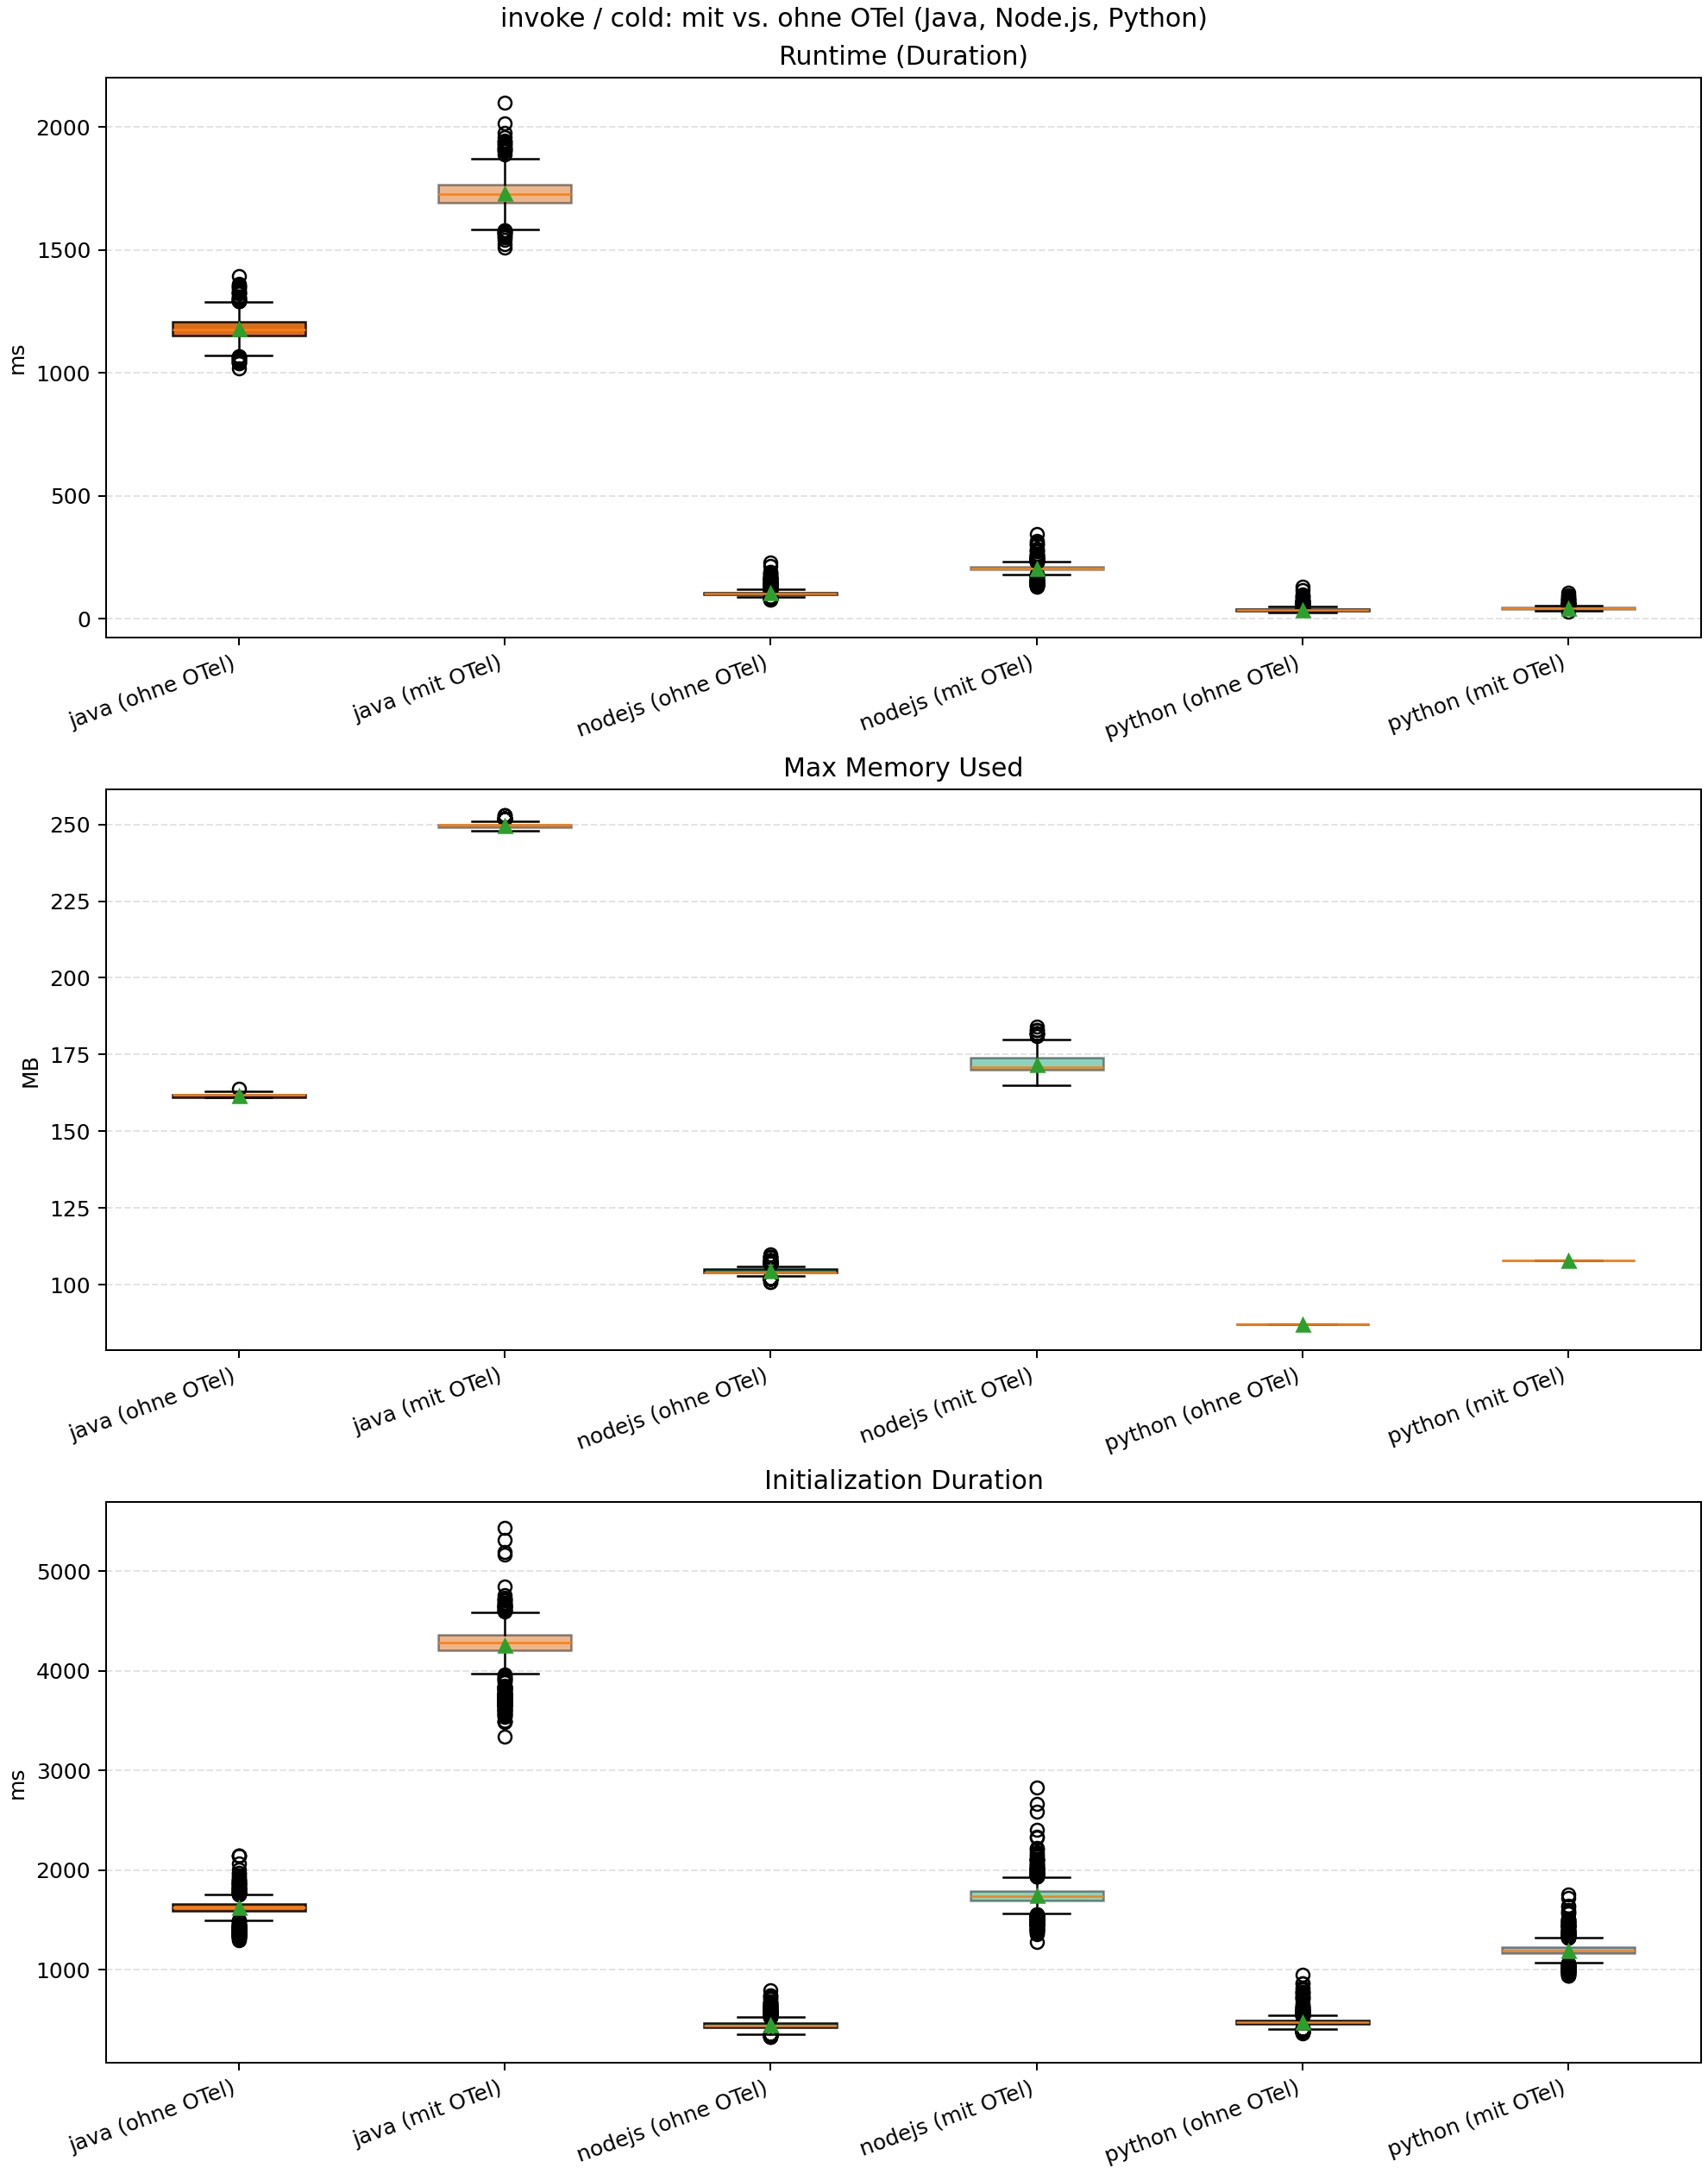
\includegraphics[width=1\textwidth]{./gfx/examples/invoke-cold-otel-comparison.png}
    \caption{Verteilung der Kaltstartergebnisse für die Lambdaverkettung.}
    \label{fig:invoke-cold-otel-comparison}
\end{figure}

\begin{figure}[H]
    \centering
    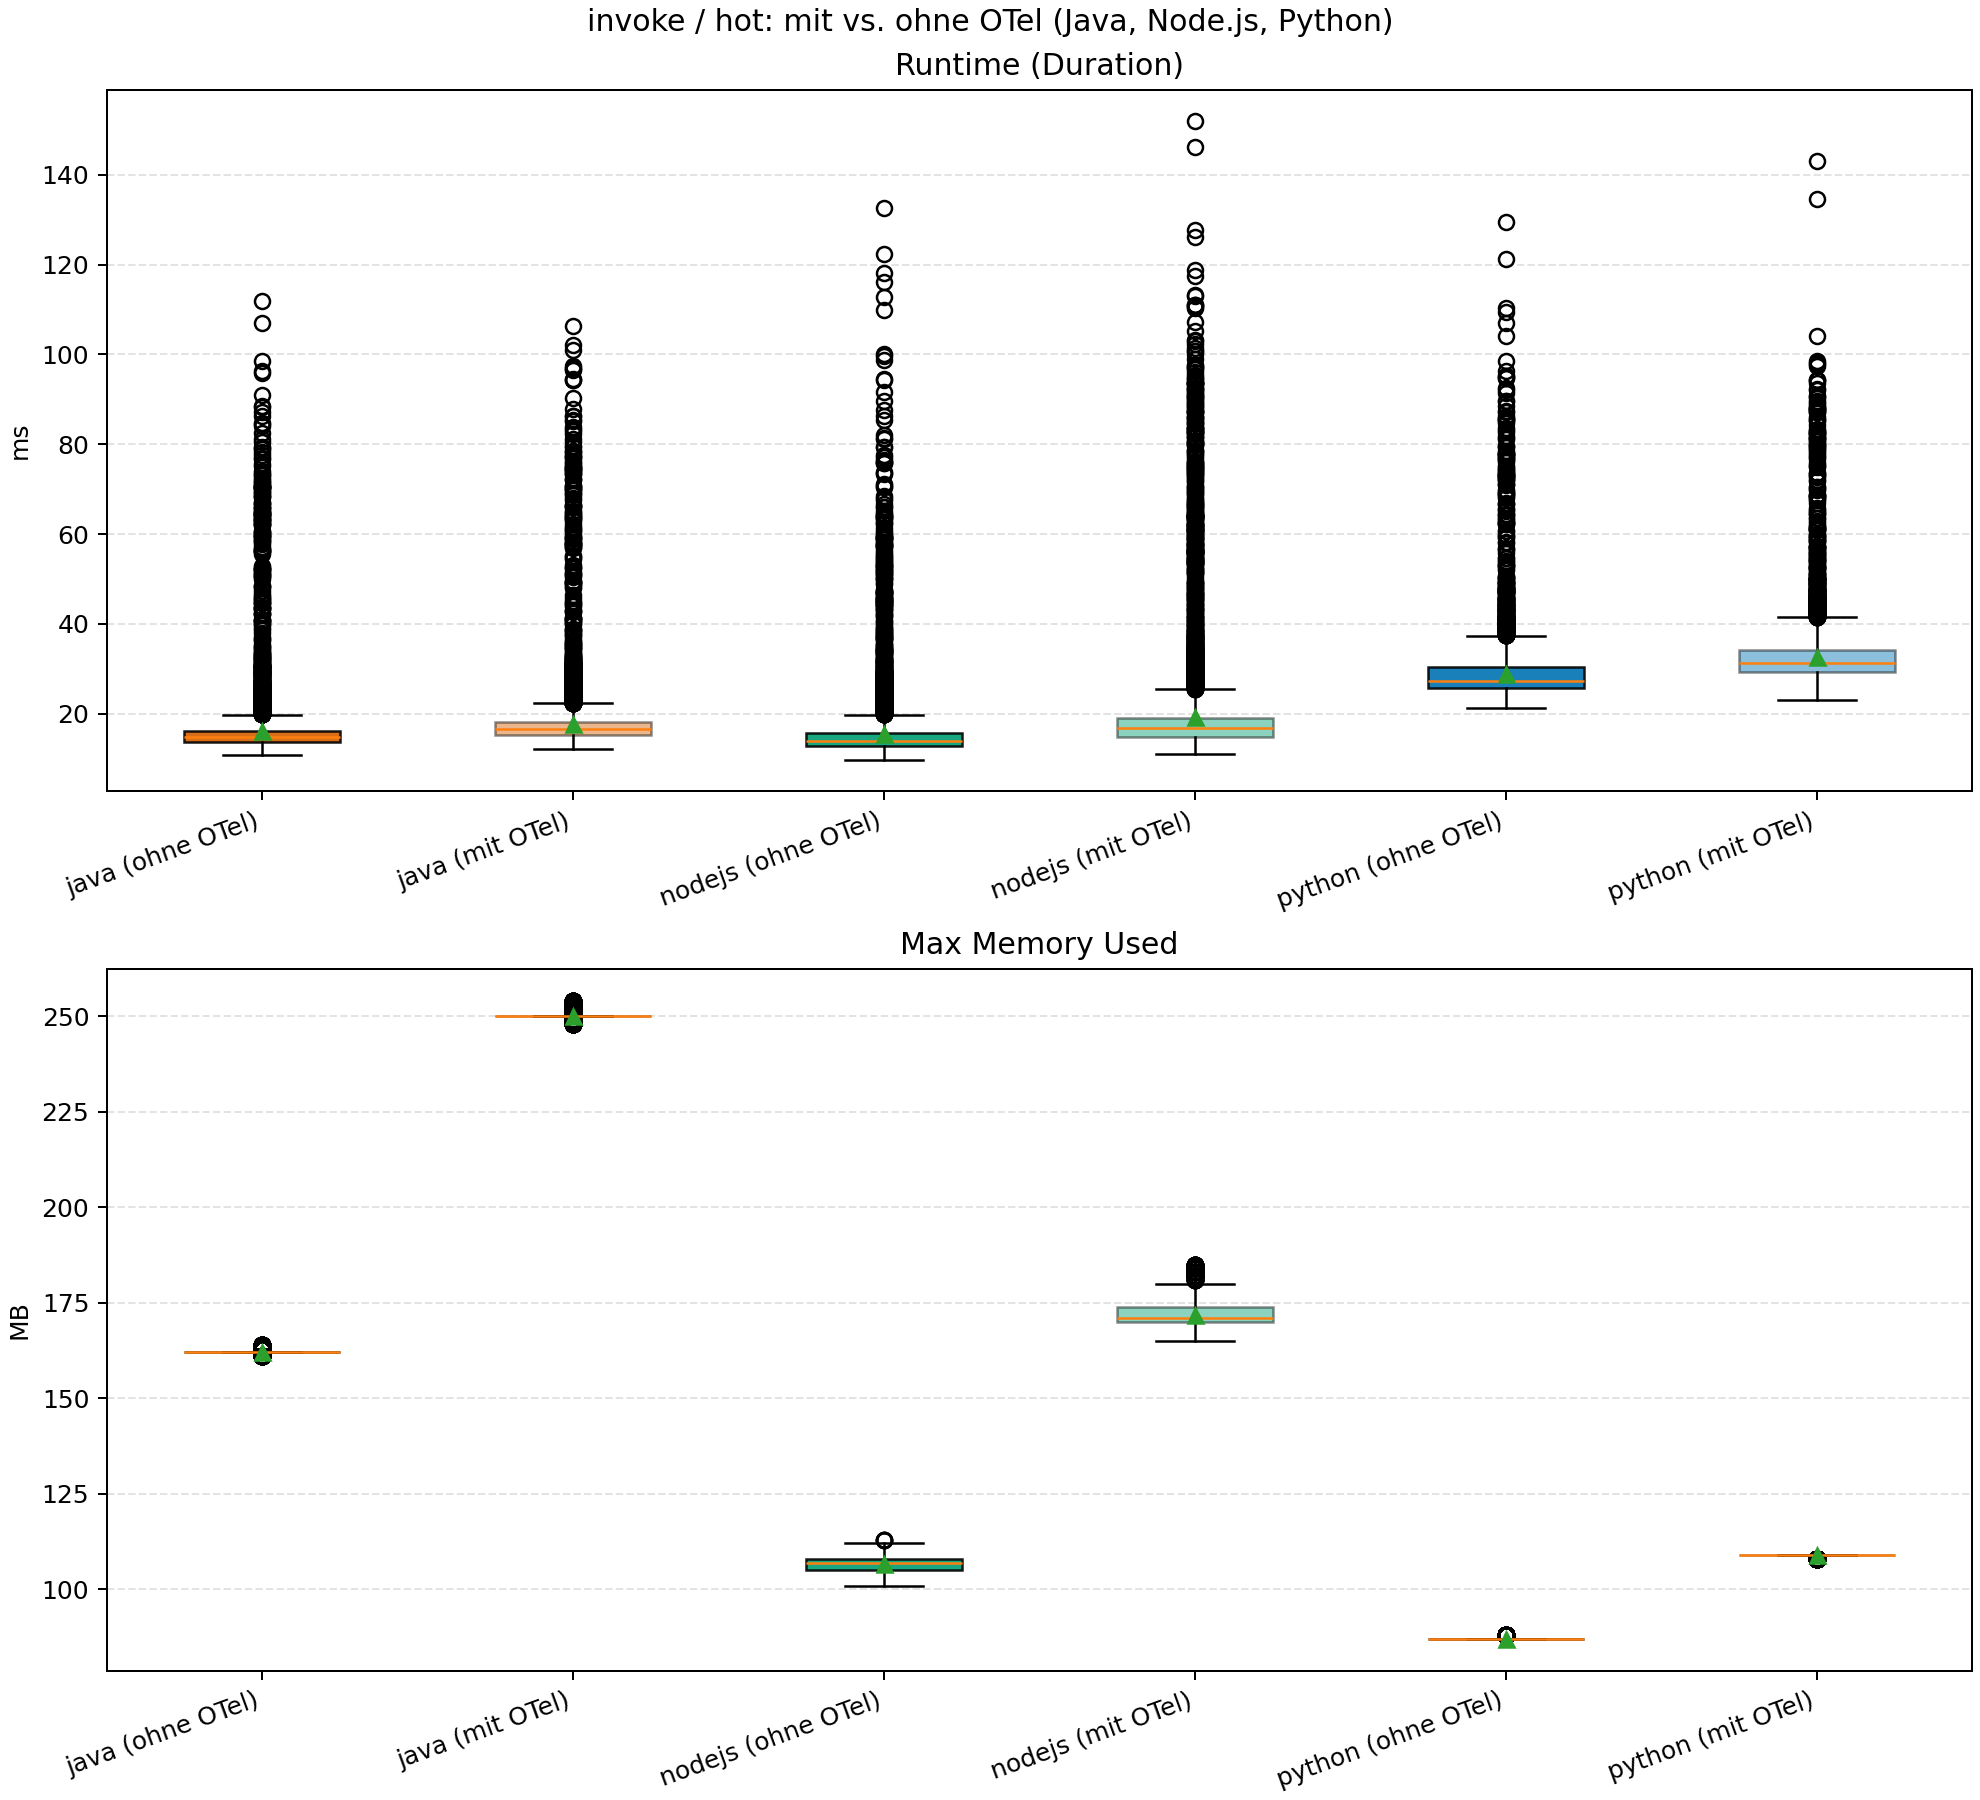
\includegraphics[width=1\textwidth]{./gfx/examples/invoke-hot-otel-comparison.png}
    \caption{Verteilung der Warmstartergebnisse für die Lambdaverkettung.}
    \label{fig:invoke-warm-otel-comparison} 
\end{figure}

\subsection{Microbenchmark 2 - HTTP-GET-Anfrage}
\begin{figure}[H]
    \centering
    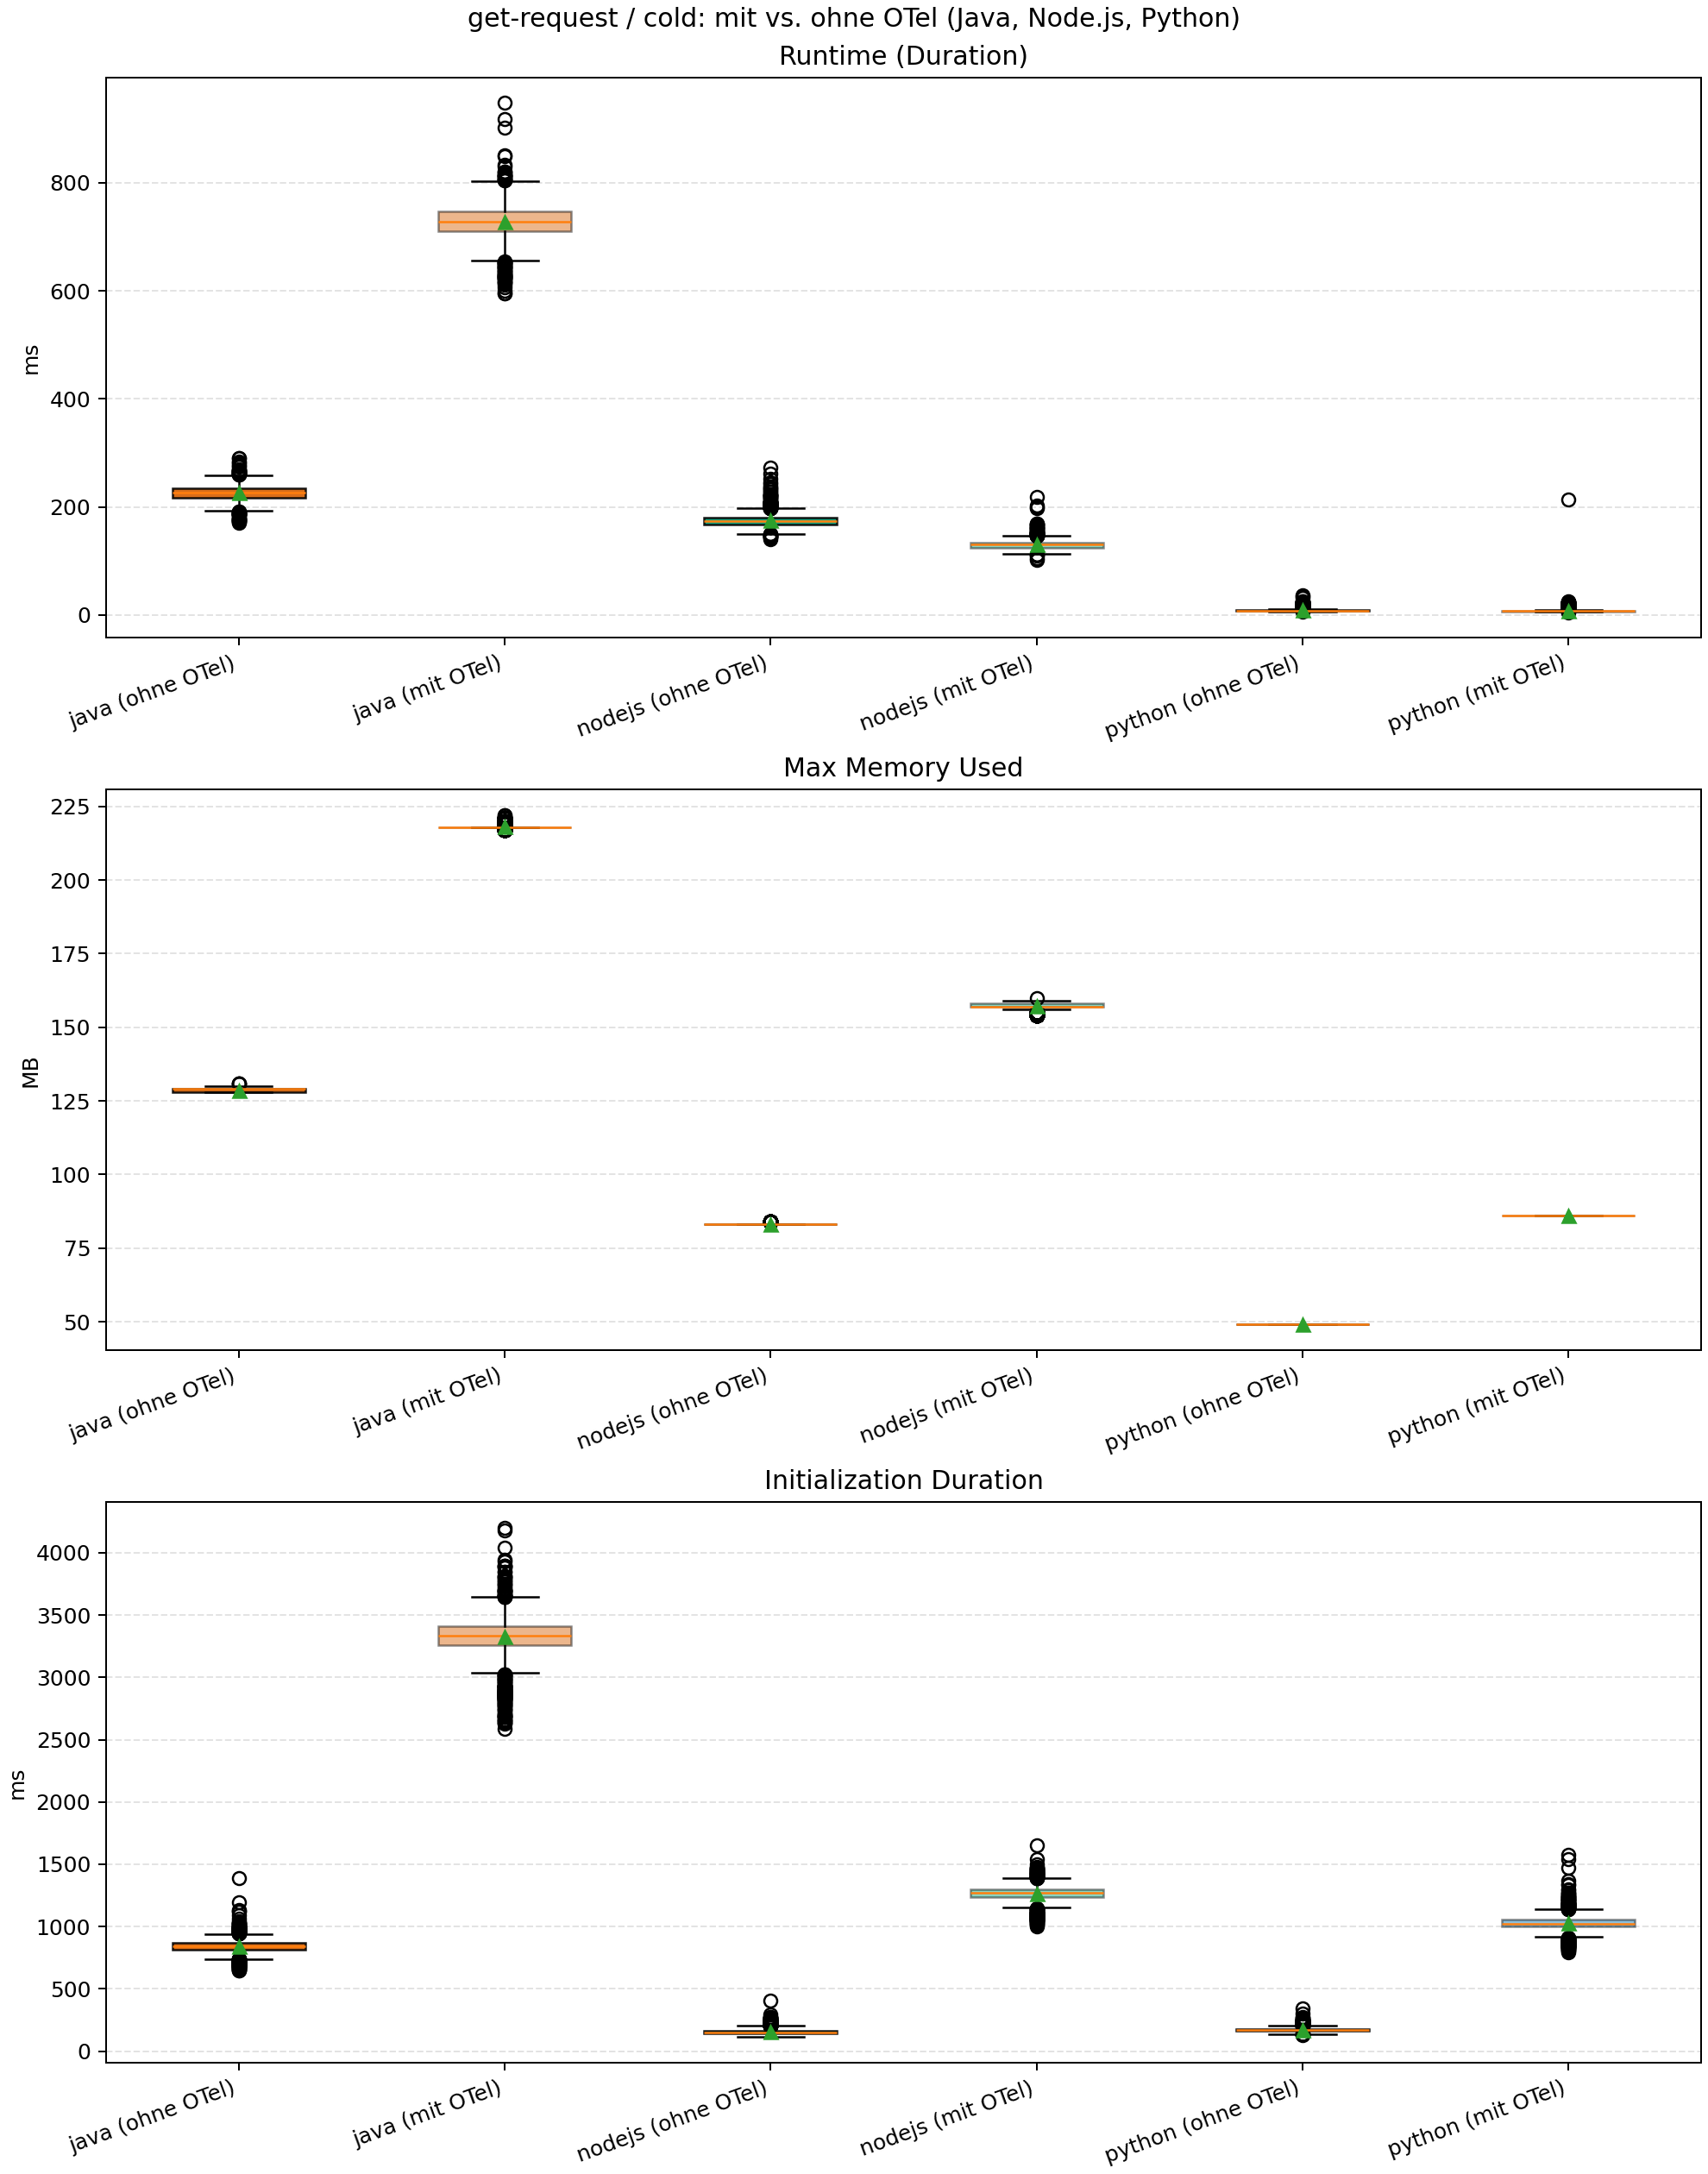
\includegraphics[width=1\textwidth]{./gfx/examples/get-request-cold-otel-comparison.png}
    \caption{Verteilung der Kaltstartergebnisse für die HTTP-GET-Anfrage.}
    \label{fig:http-get-cold-otel-comparison}
\end{figure}
\begin{figure}[H]
    \centering
    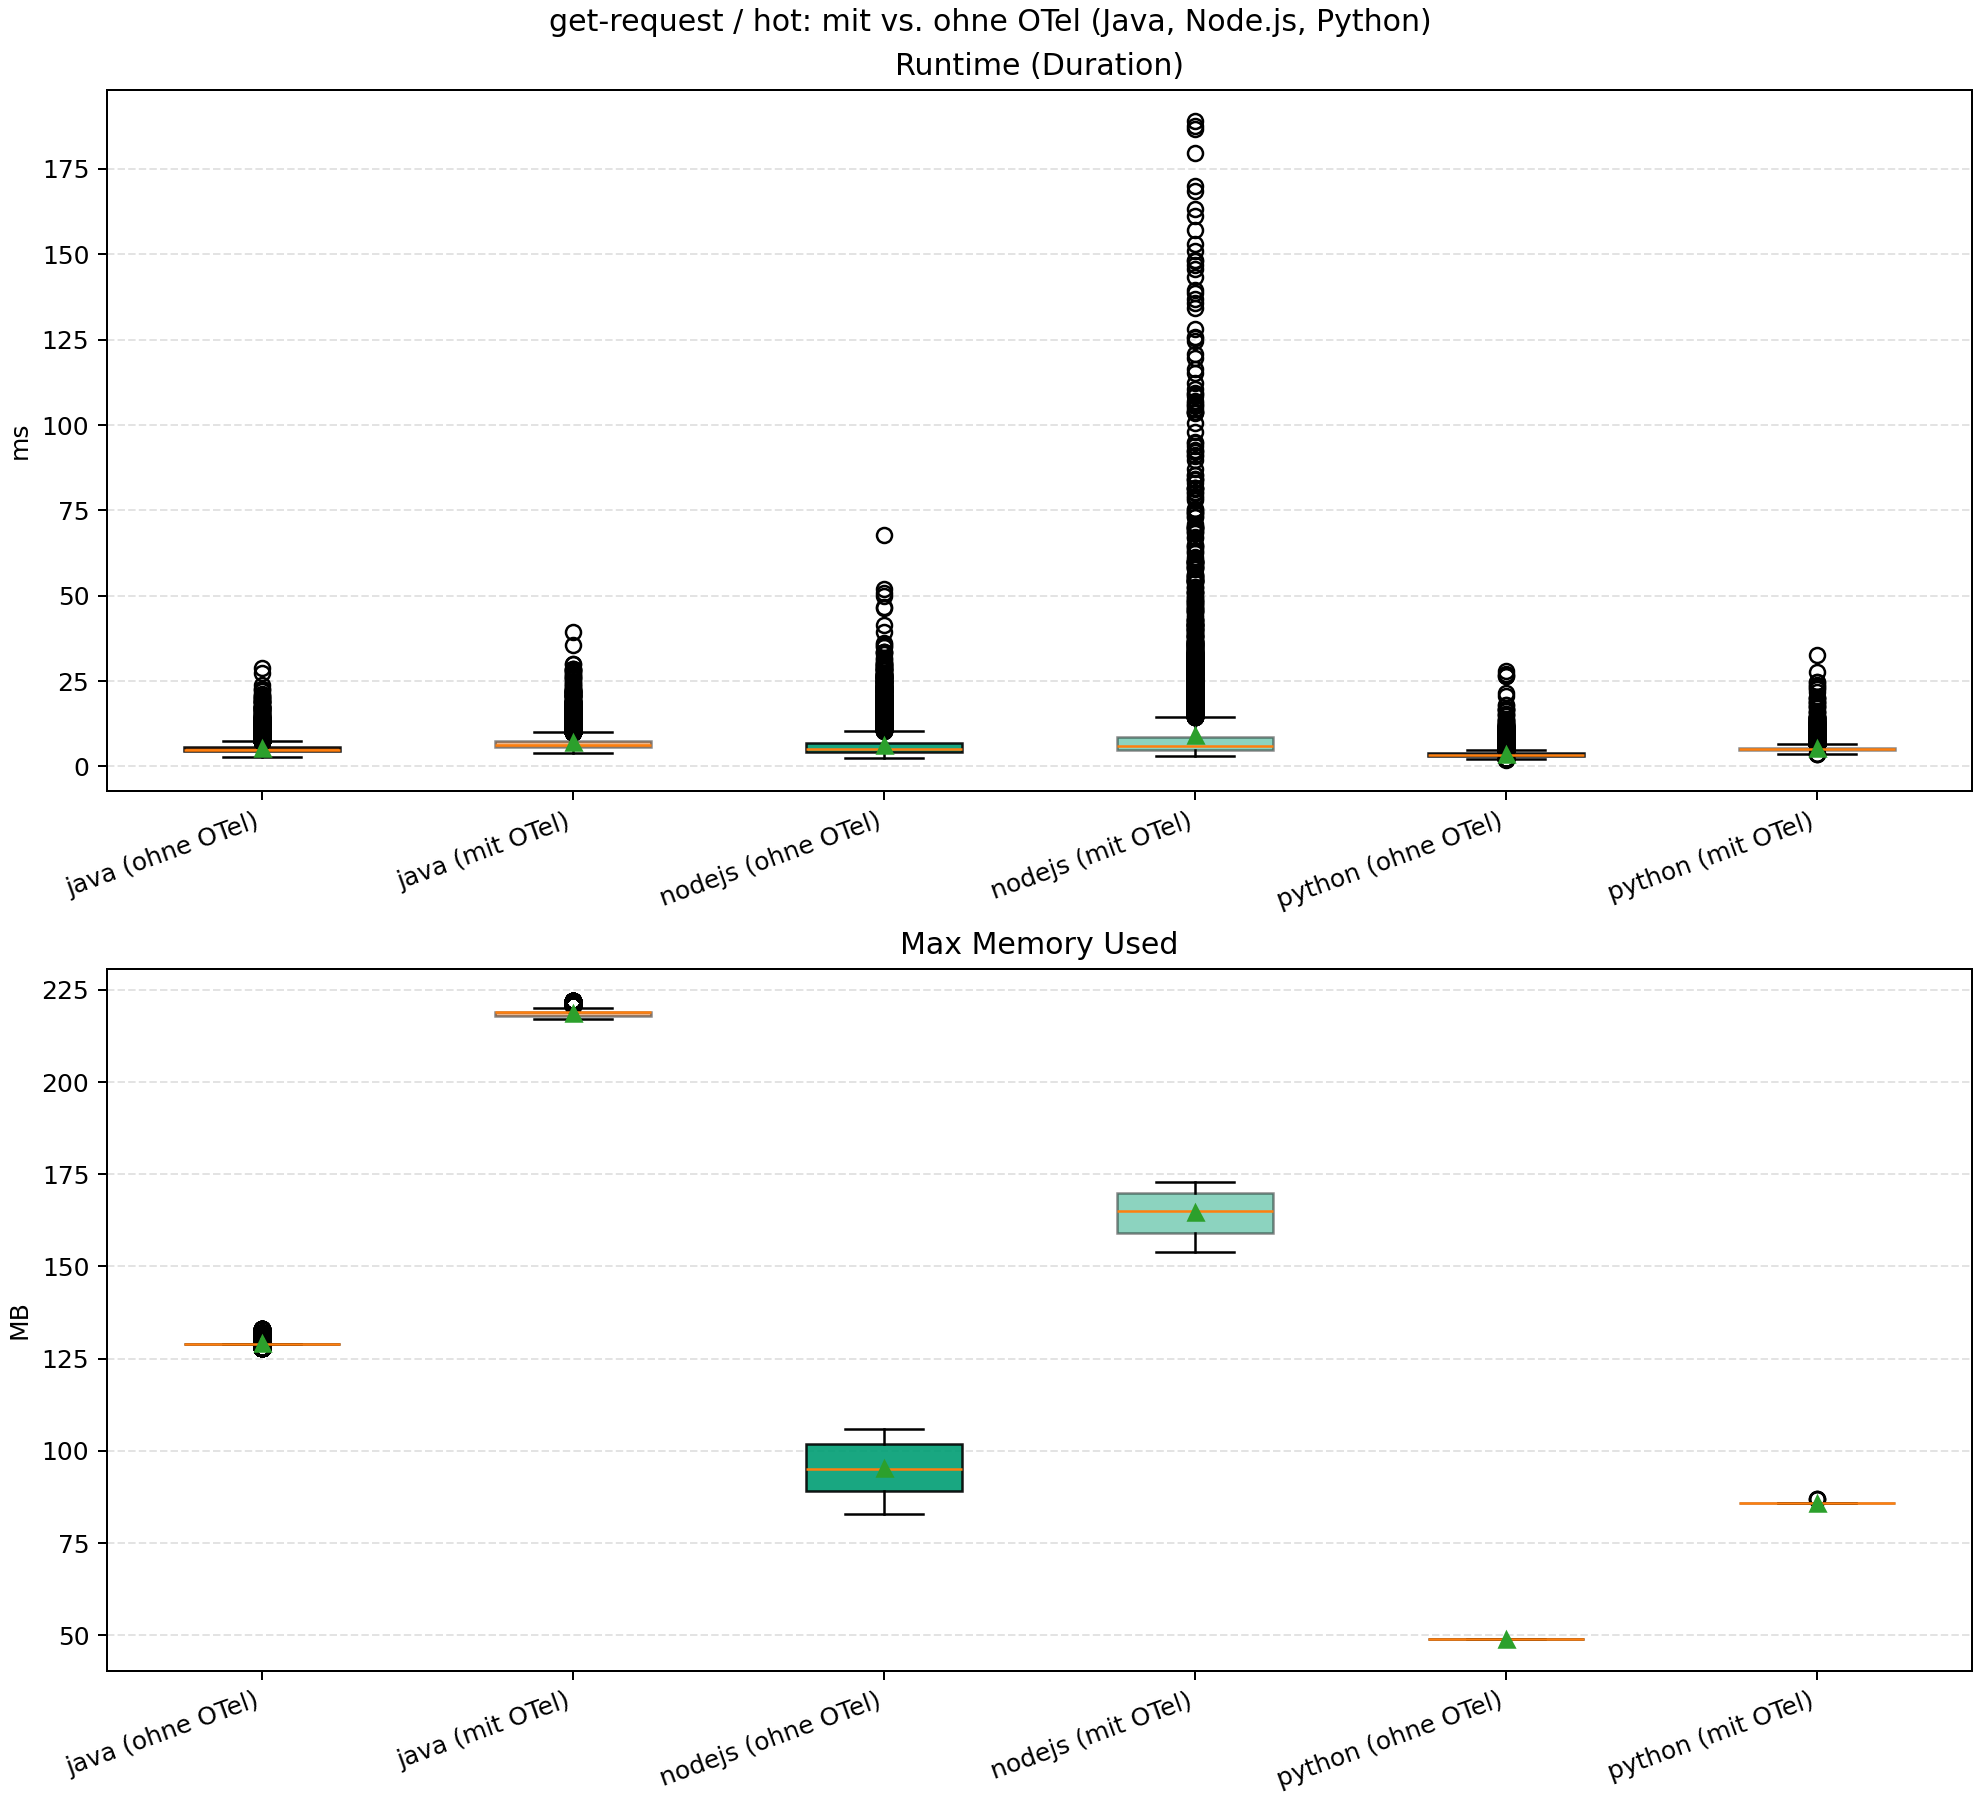
\includegraphics[width=1\textwidth]{./gfx/examples/get-request-hot-otel-comparison.png}
    \caption{Verteilung der Warmstartergebnisse für die HTTP-GET-Anfrage.}
    \label{fig:http-get-hot-otel-comparison}
\end{figure}

\subsection{Microbenchmark 3 - HTTP-POST-Anfrage}

\begin{figure}[H]
    \centering
    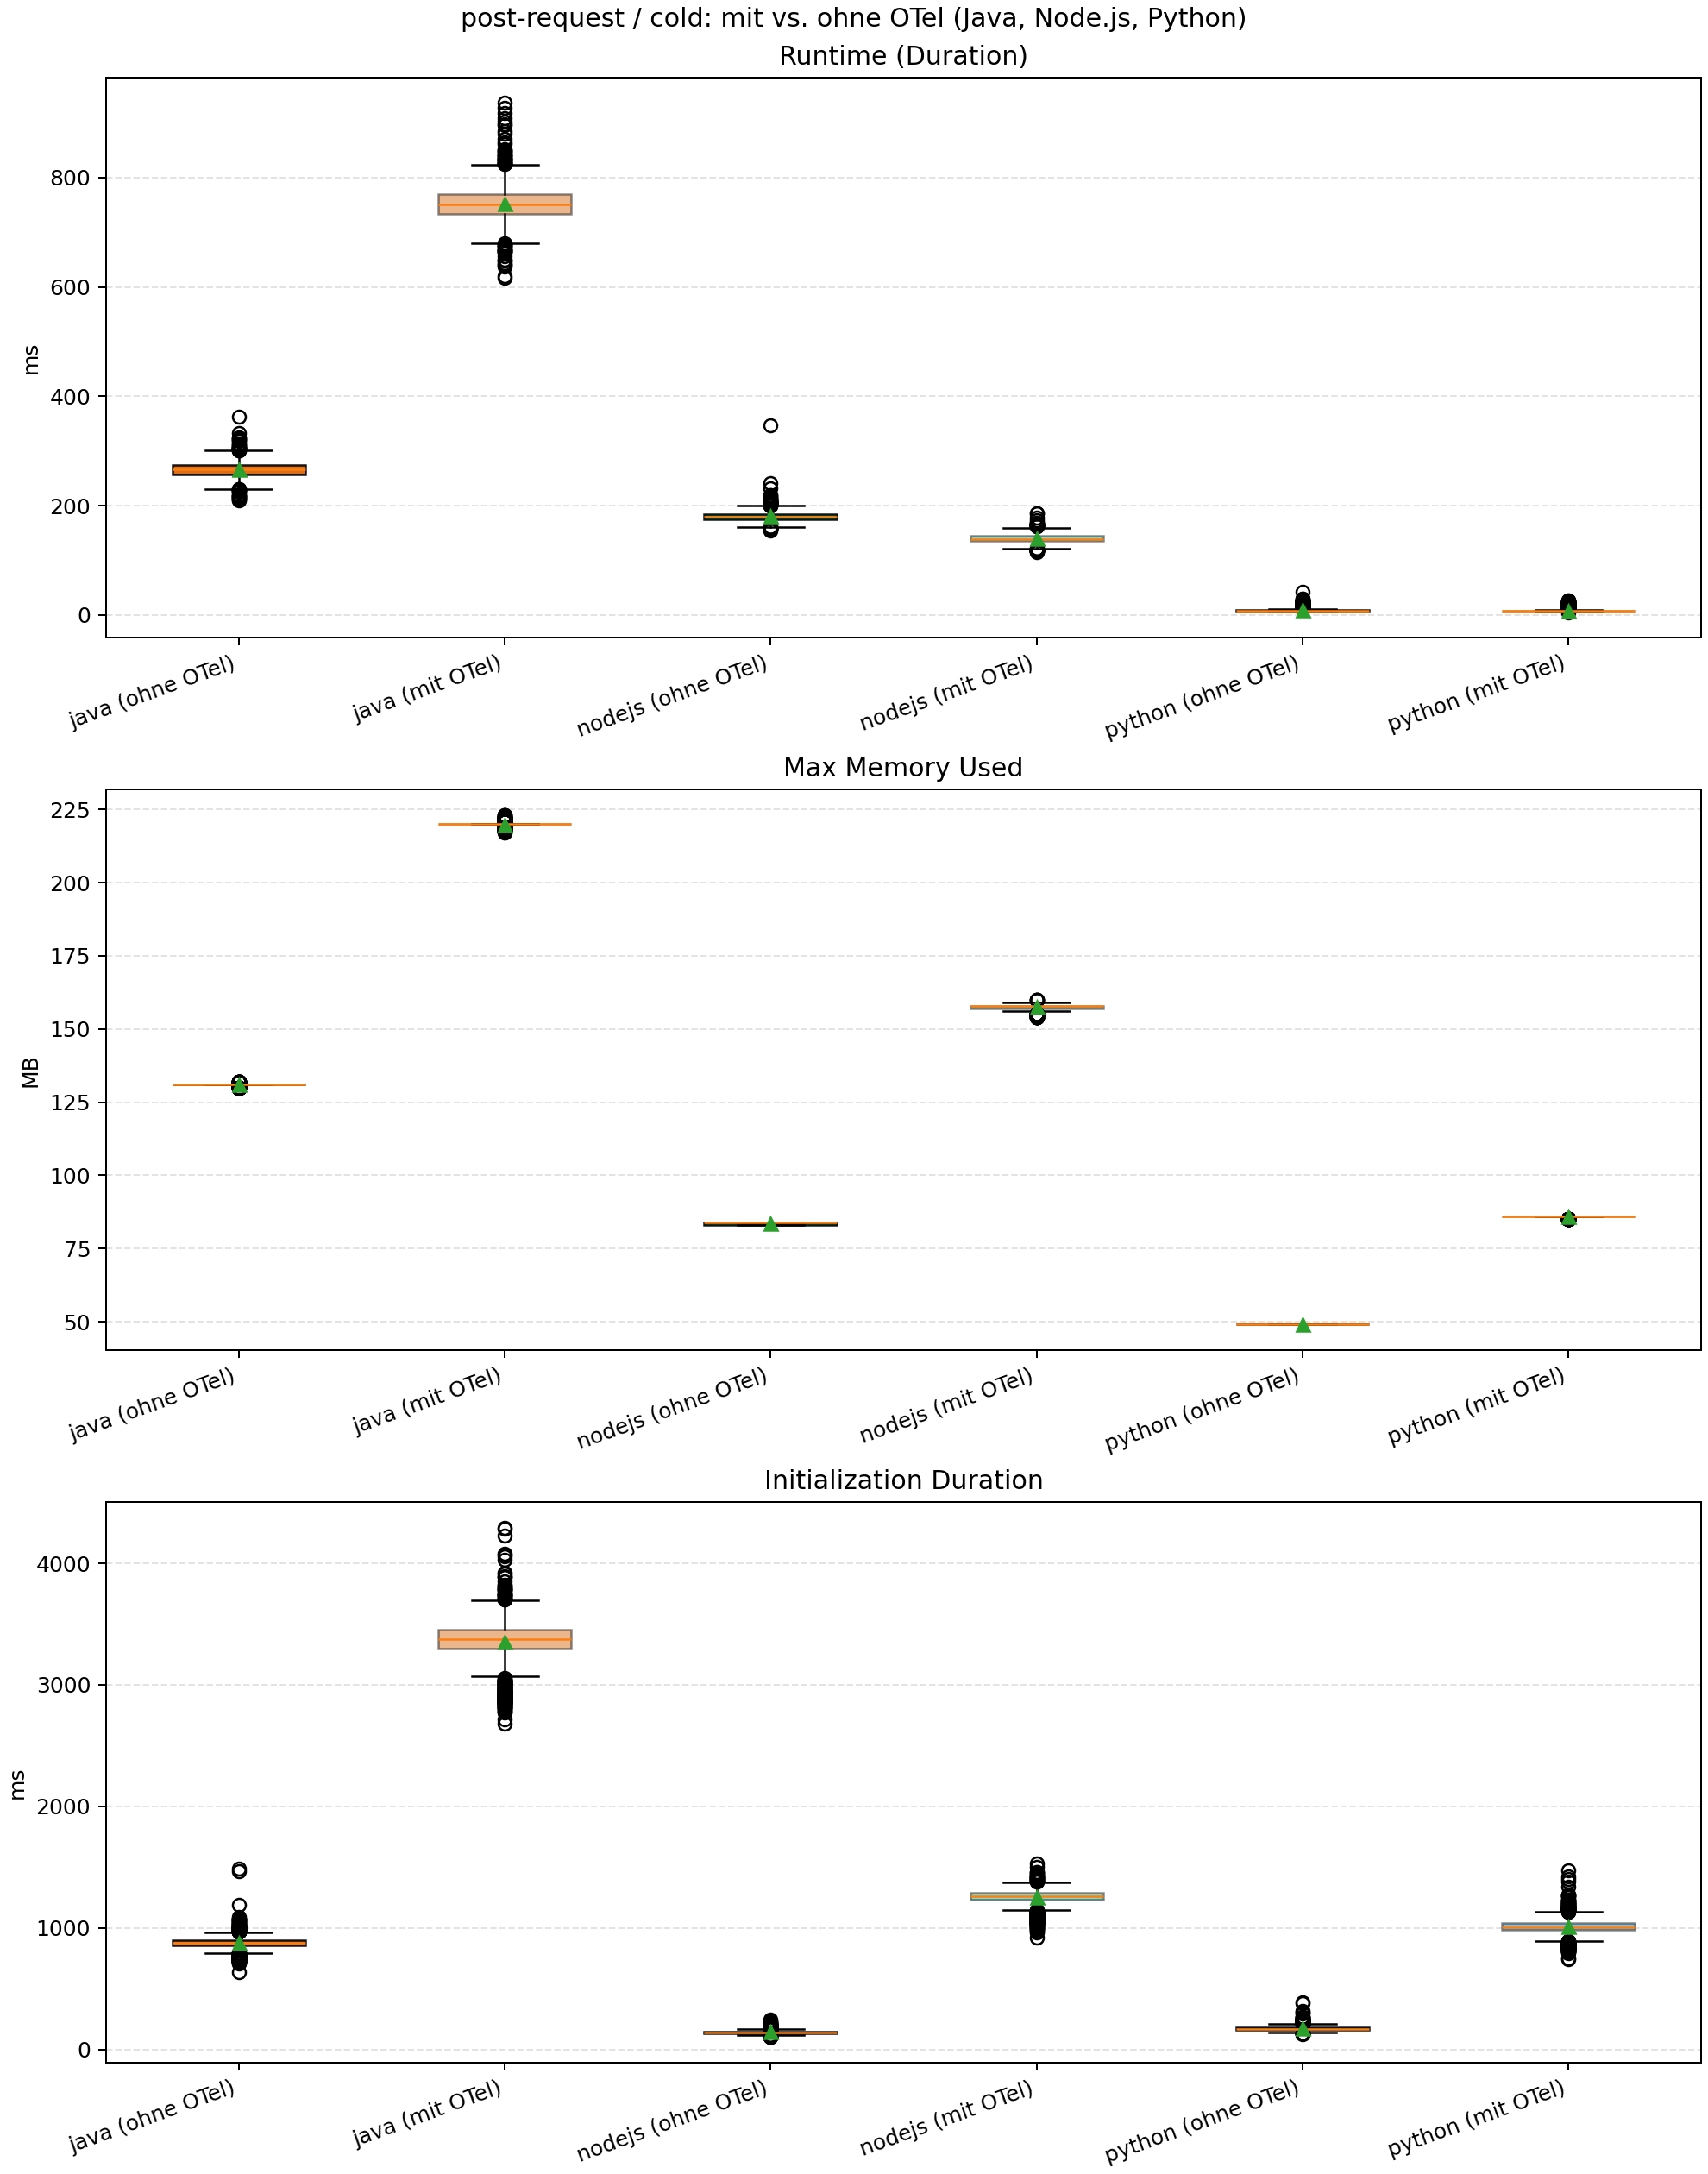
\includegraphics[width=1\textwidth]{./gfx/examples/post-request-cold-otel-comparison.png}
    \caption{Verteilung der Kaltstartergebnisse für die HTTP-POST-Anfrage.}
    \label{fig:http-post-cold-otel-comparison}
\end{figure}

\begin{figure}[H]
    \centering
    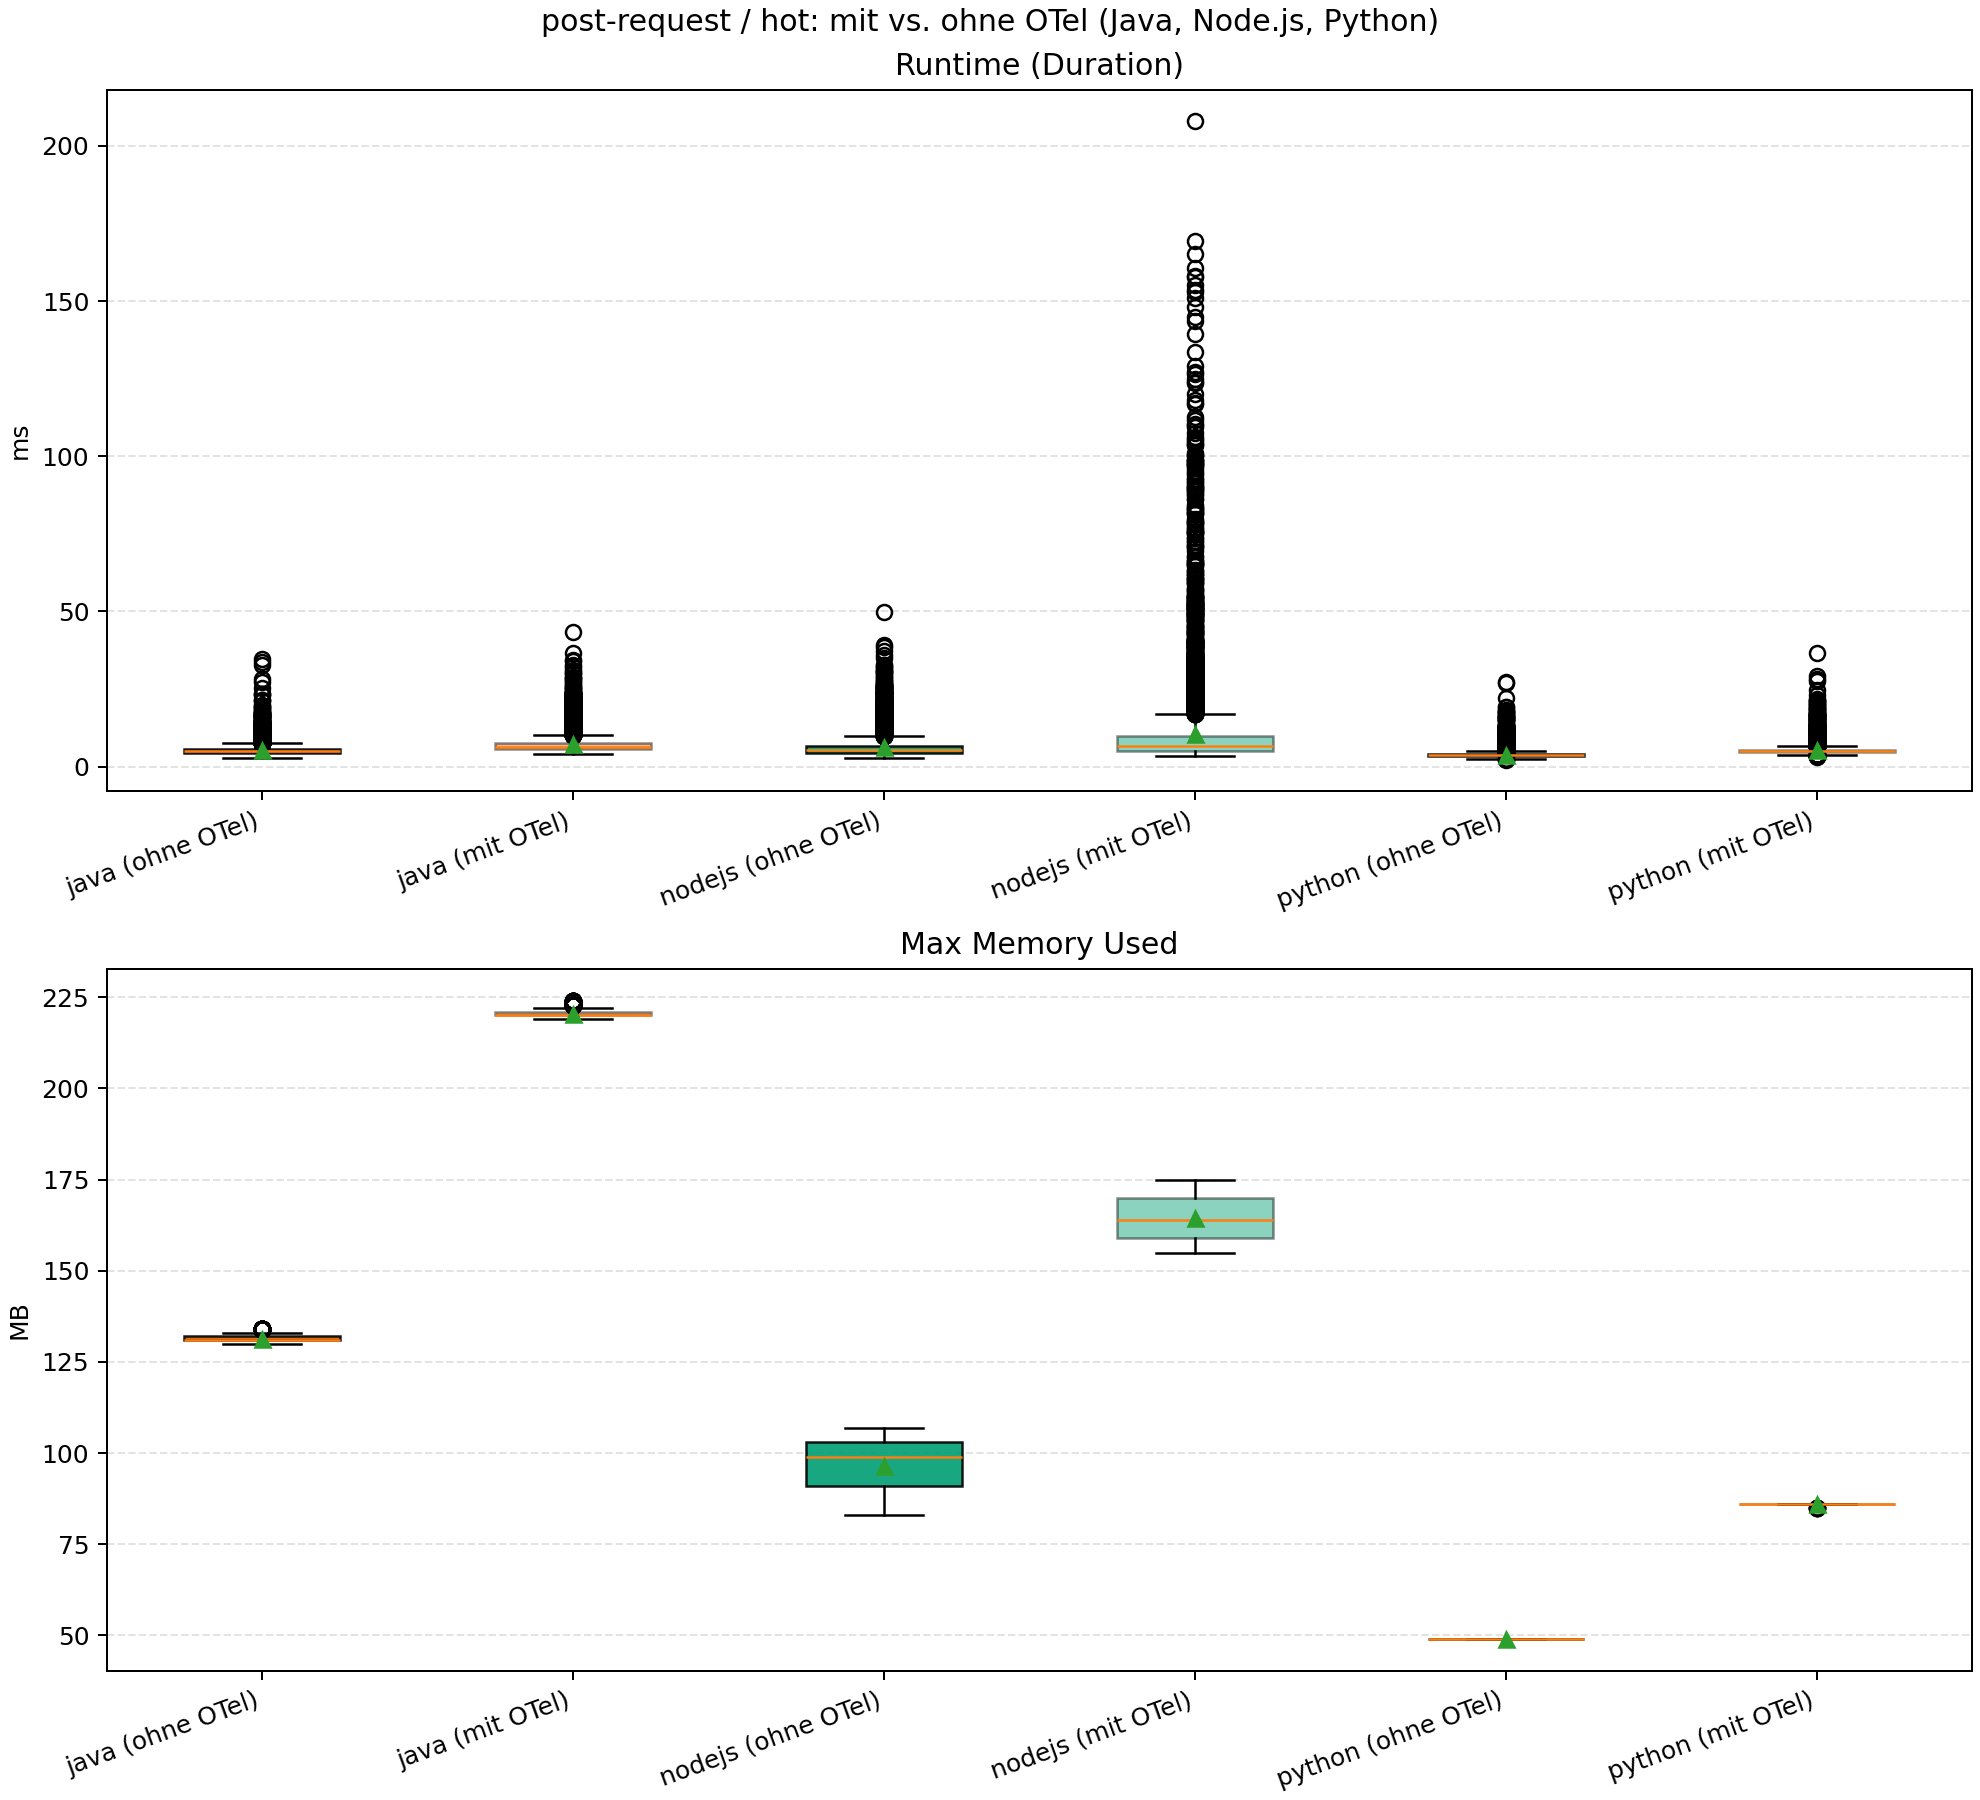
\includegraphics[width=1\textwidth]{./gfx/examples/post-request-hot-otel-comparison.png}
    \caption{Verteilung der Warmstartergebnisse für die HTTP-POST-Anfrage.}
    \label{fig:http-post-hot-otel-comparison}
\end{figure}

\subsection{Microbenchmark 4 - DynamoDB-Leseoperation}

\begin{figure}[H]
    \centering
    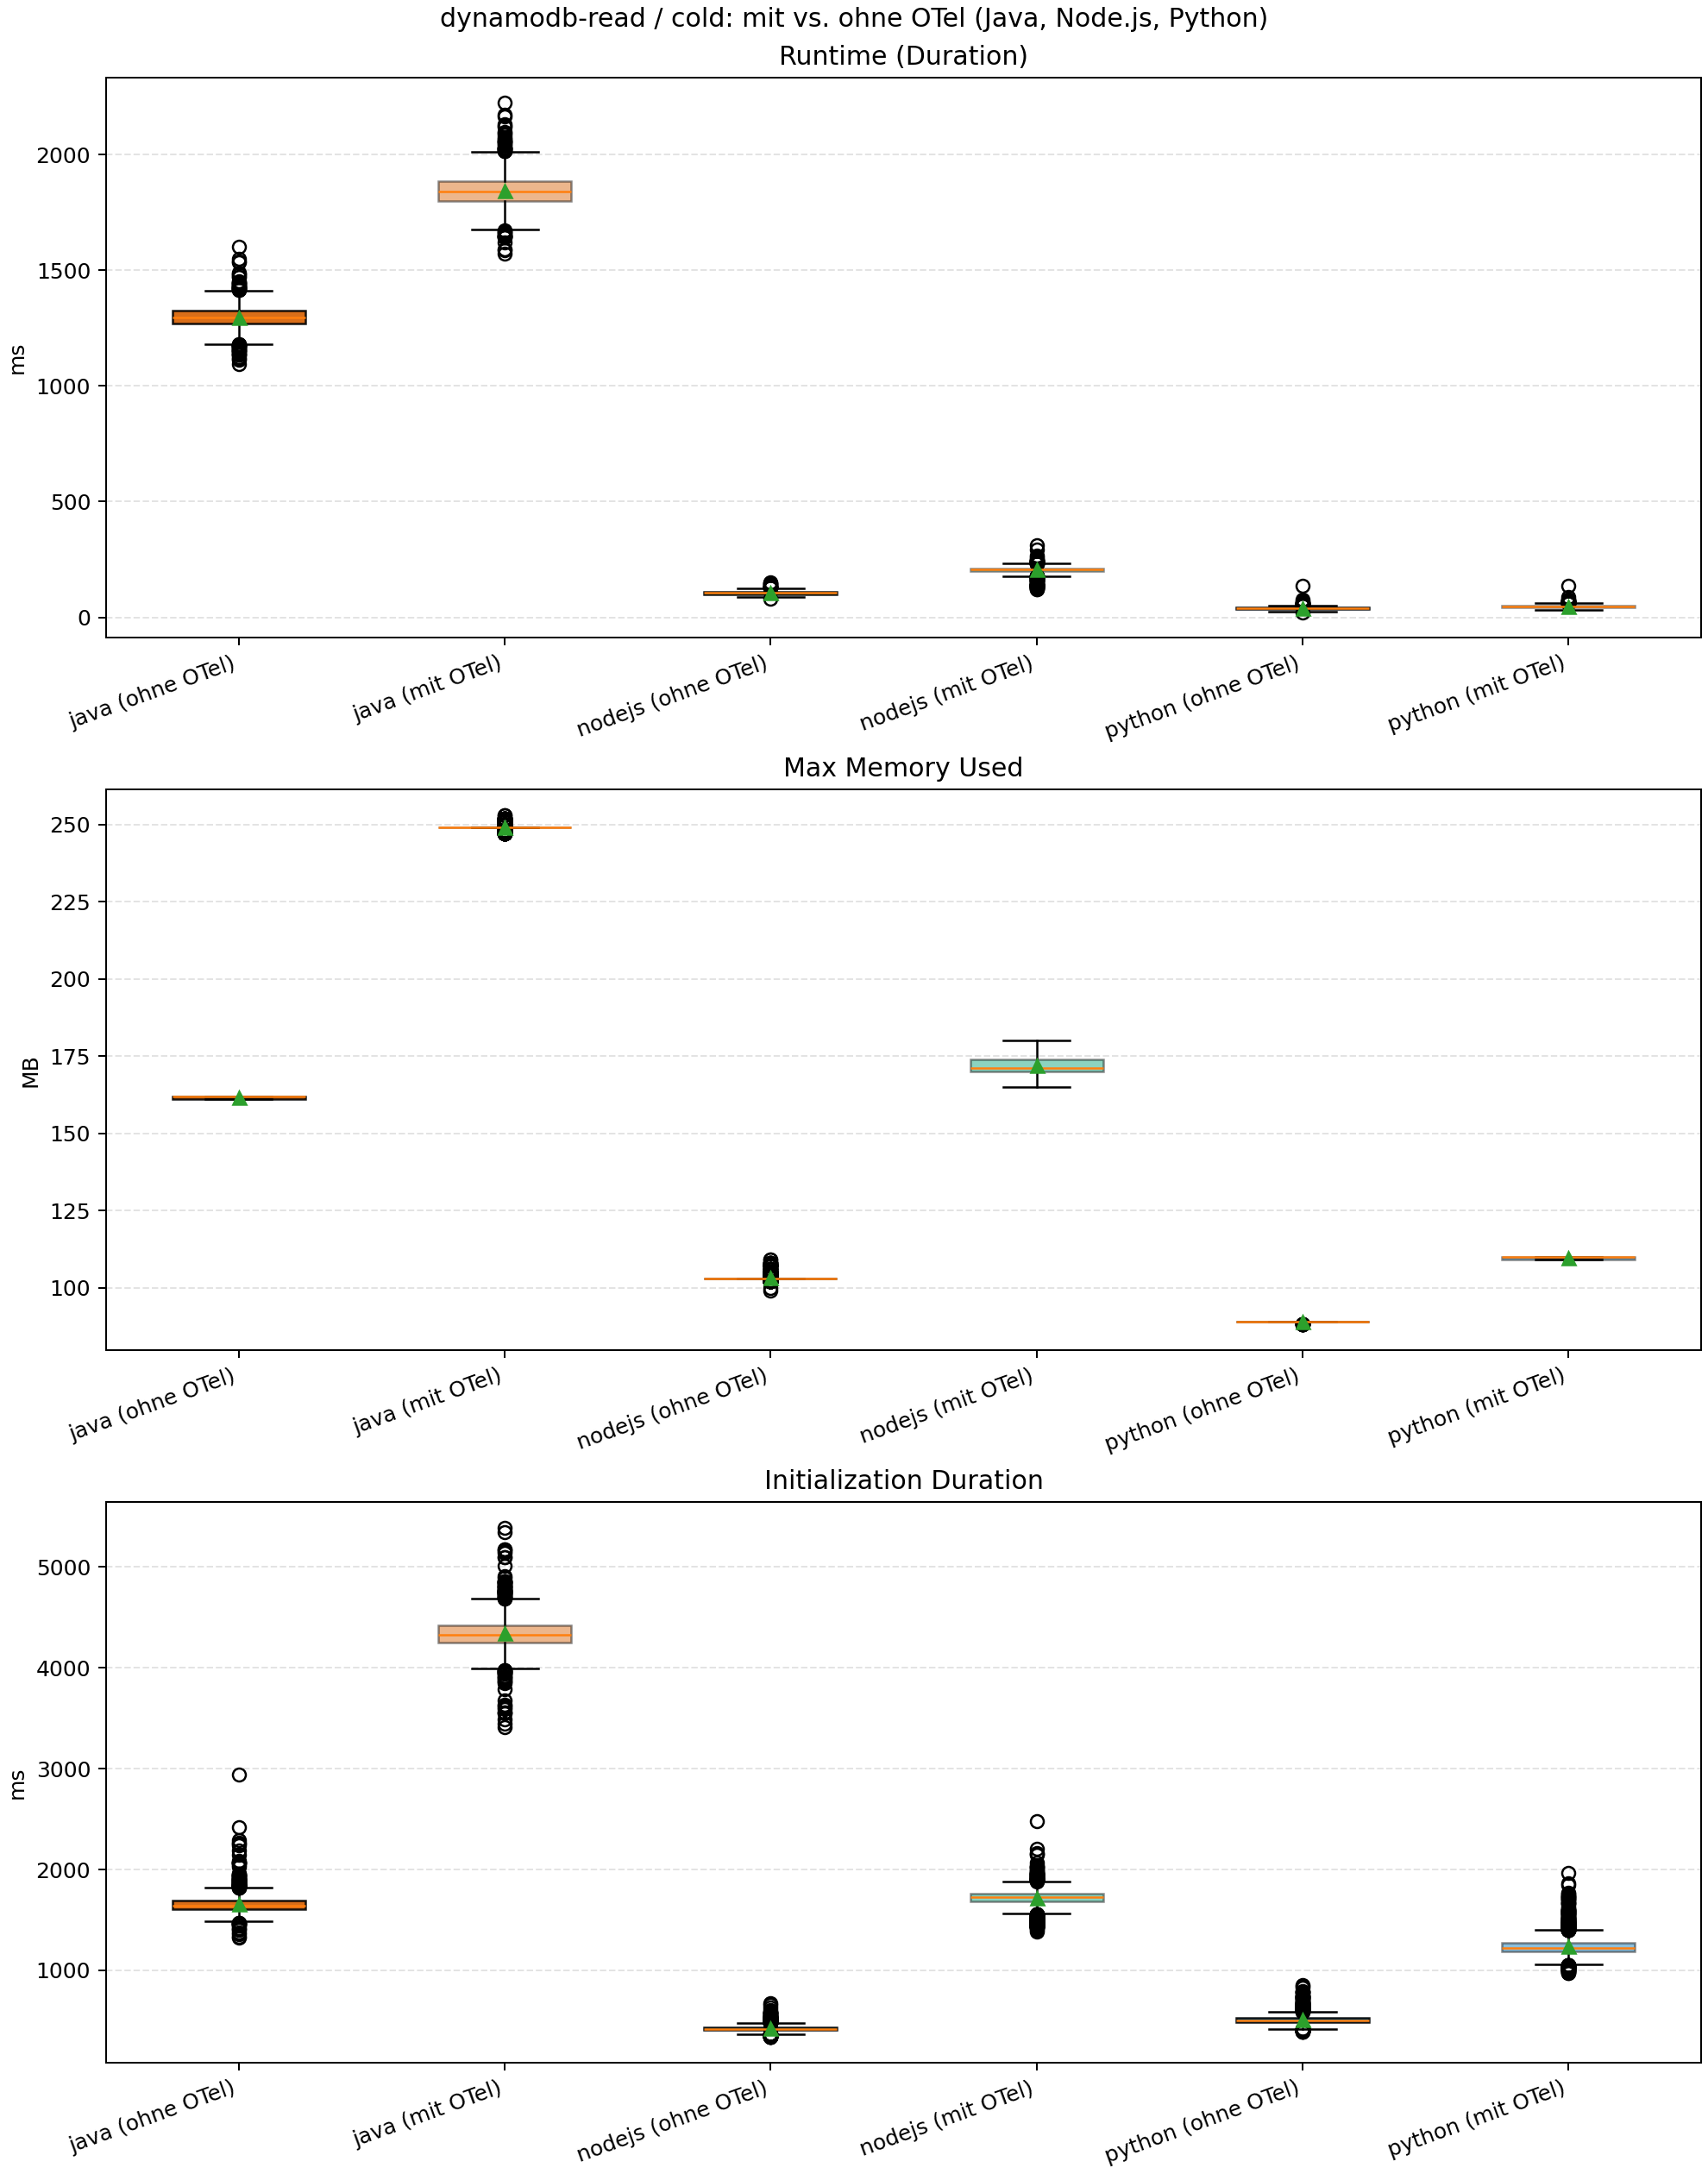
\includegraphics[width=1\textwidth]{./gfx/examples/dynamodb-read-cold-otel-comparison.png}
    \caption{Verteilung der Kaltstartergebnisse für die DynamoDB-Leseoperation.}
    \label{fig:dynamodb-read-cold-otel-comparison}
\end{figure}

\begin{figure}[H]
    \centering
    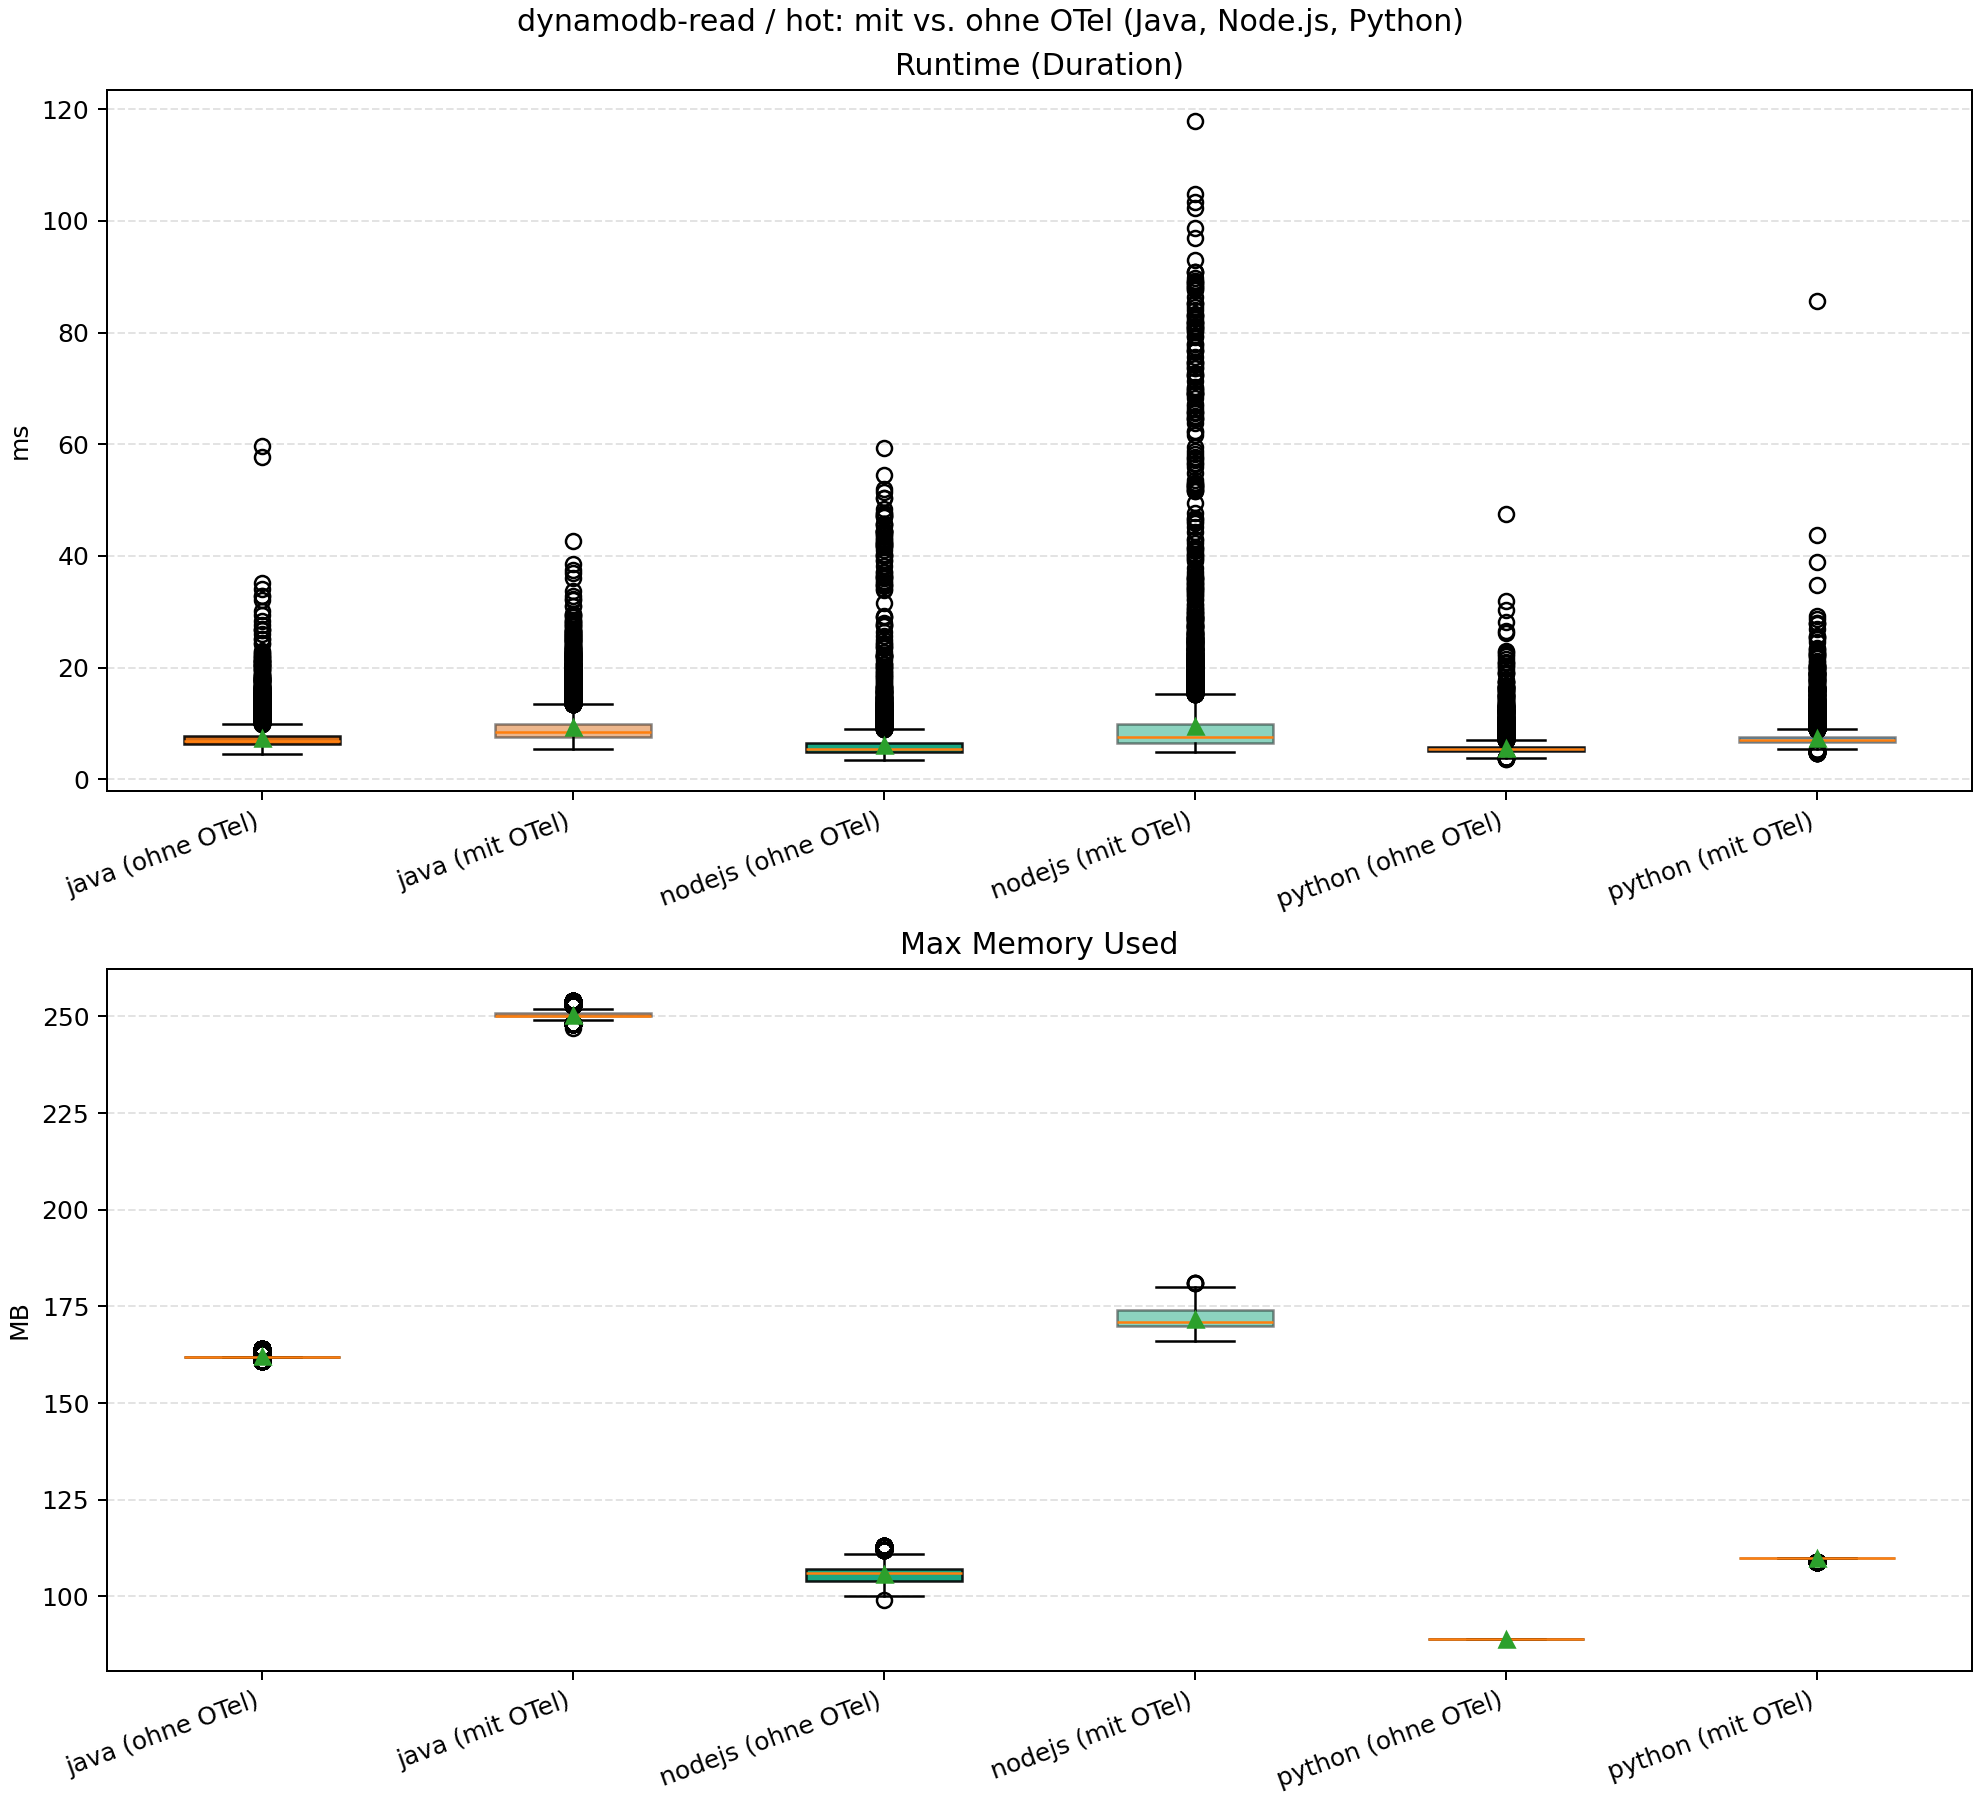
\includegraphics[width=1\textwidth]{./gfx/examples/dynamodb-read-hot-otel-comparison.png}
    \caption{Verteilung der Warmstartergebnisse für die DynamoDB-Leseoperation.}
    \label{fig:dynamodb-read-hot-otel-comparison}
\end{figure}

\subsection{Microbenchmark 5 - DynamoDB-Schreibeoperation}

\begin{figure}[H]
    \centering
    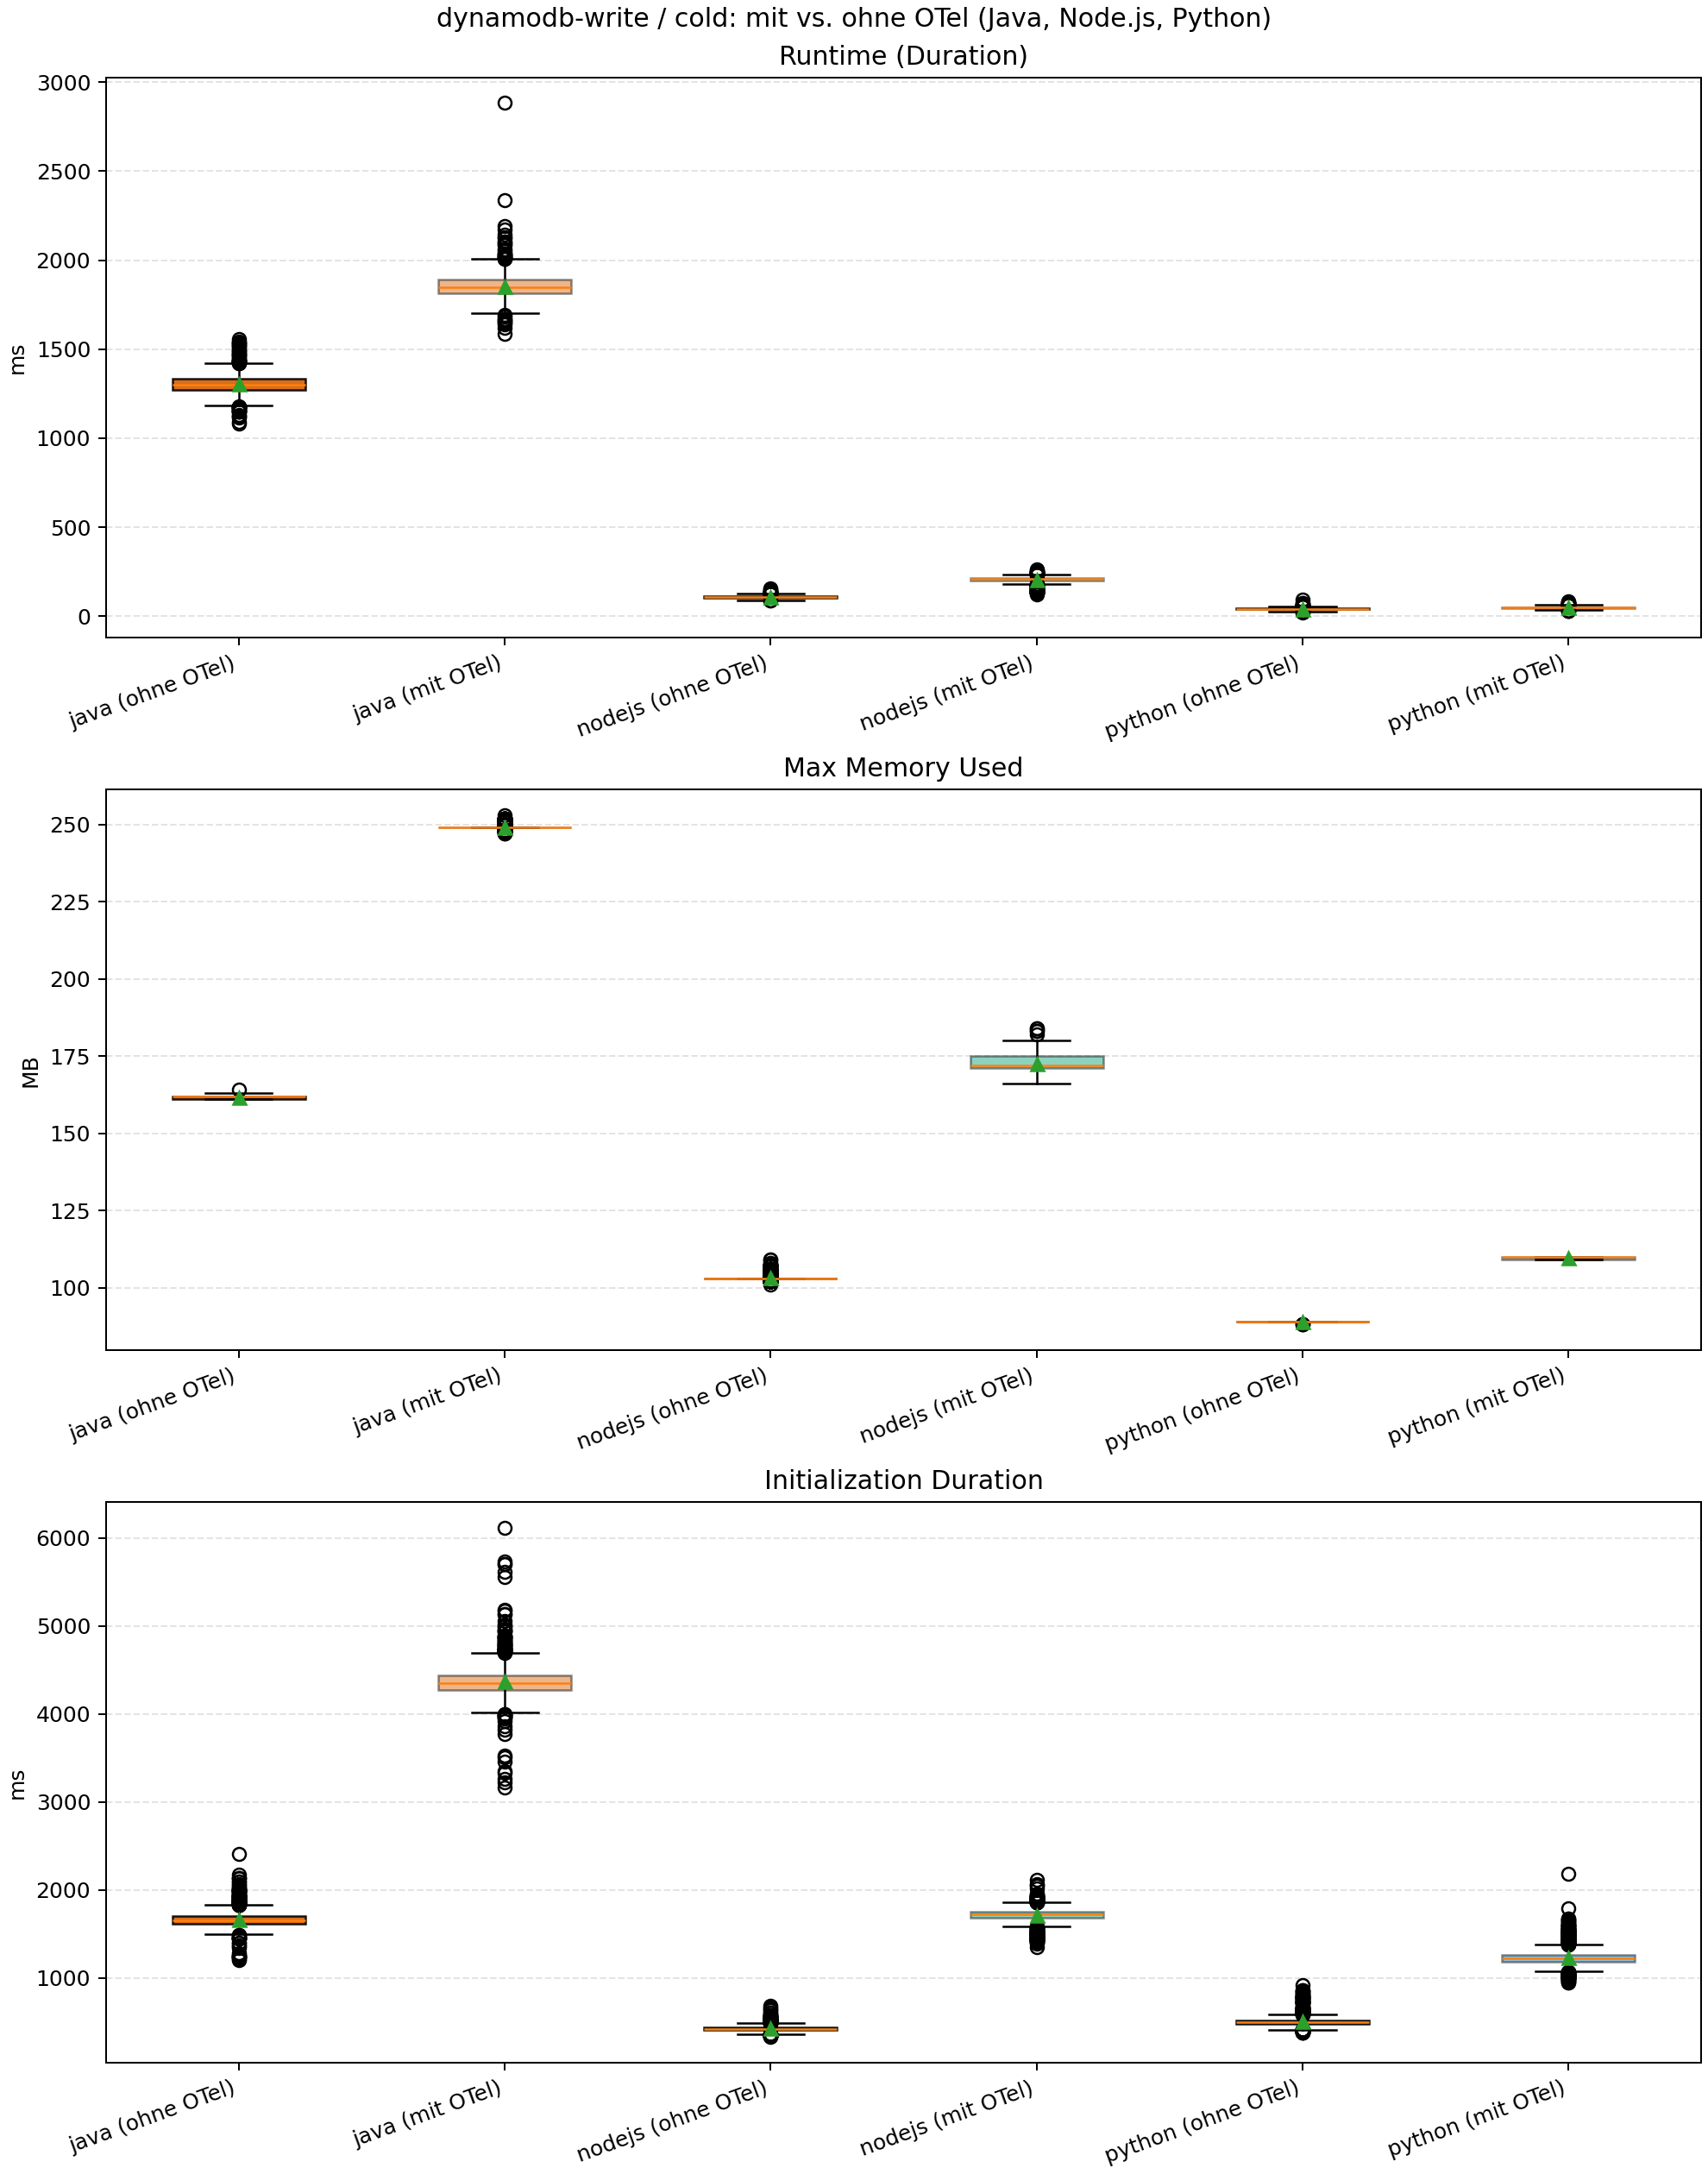
\includegraphics[width=1\textwidth]{./gfx/examples/dynamodb-write-cold-otel-comparison.png}
    \caption{Verteilung der Kaltstartergebnisse für die DynamoDB-Schreibeoperation.}
    \label{fig:dynamodb-write-cold-otel-comparison}
\end{figure}

\begin{figure}[H]
    \centering
    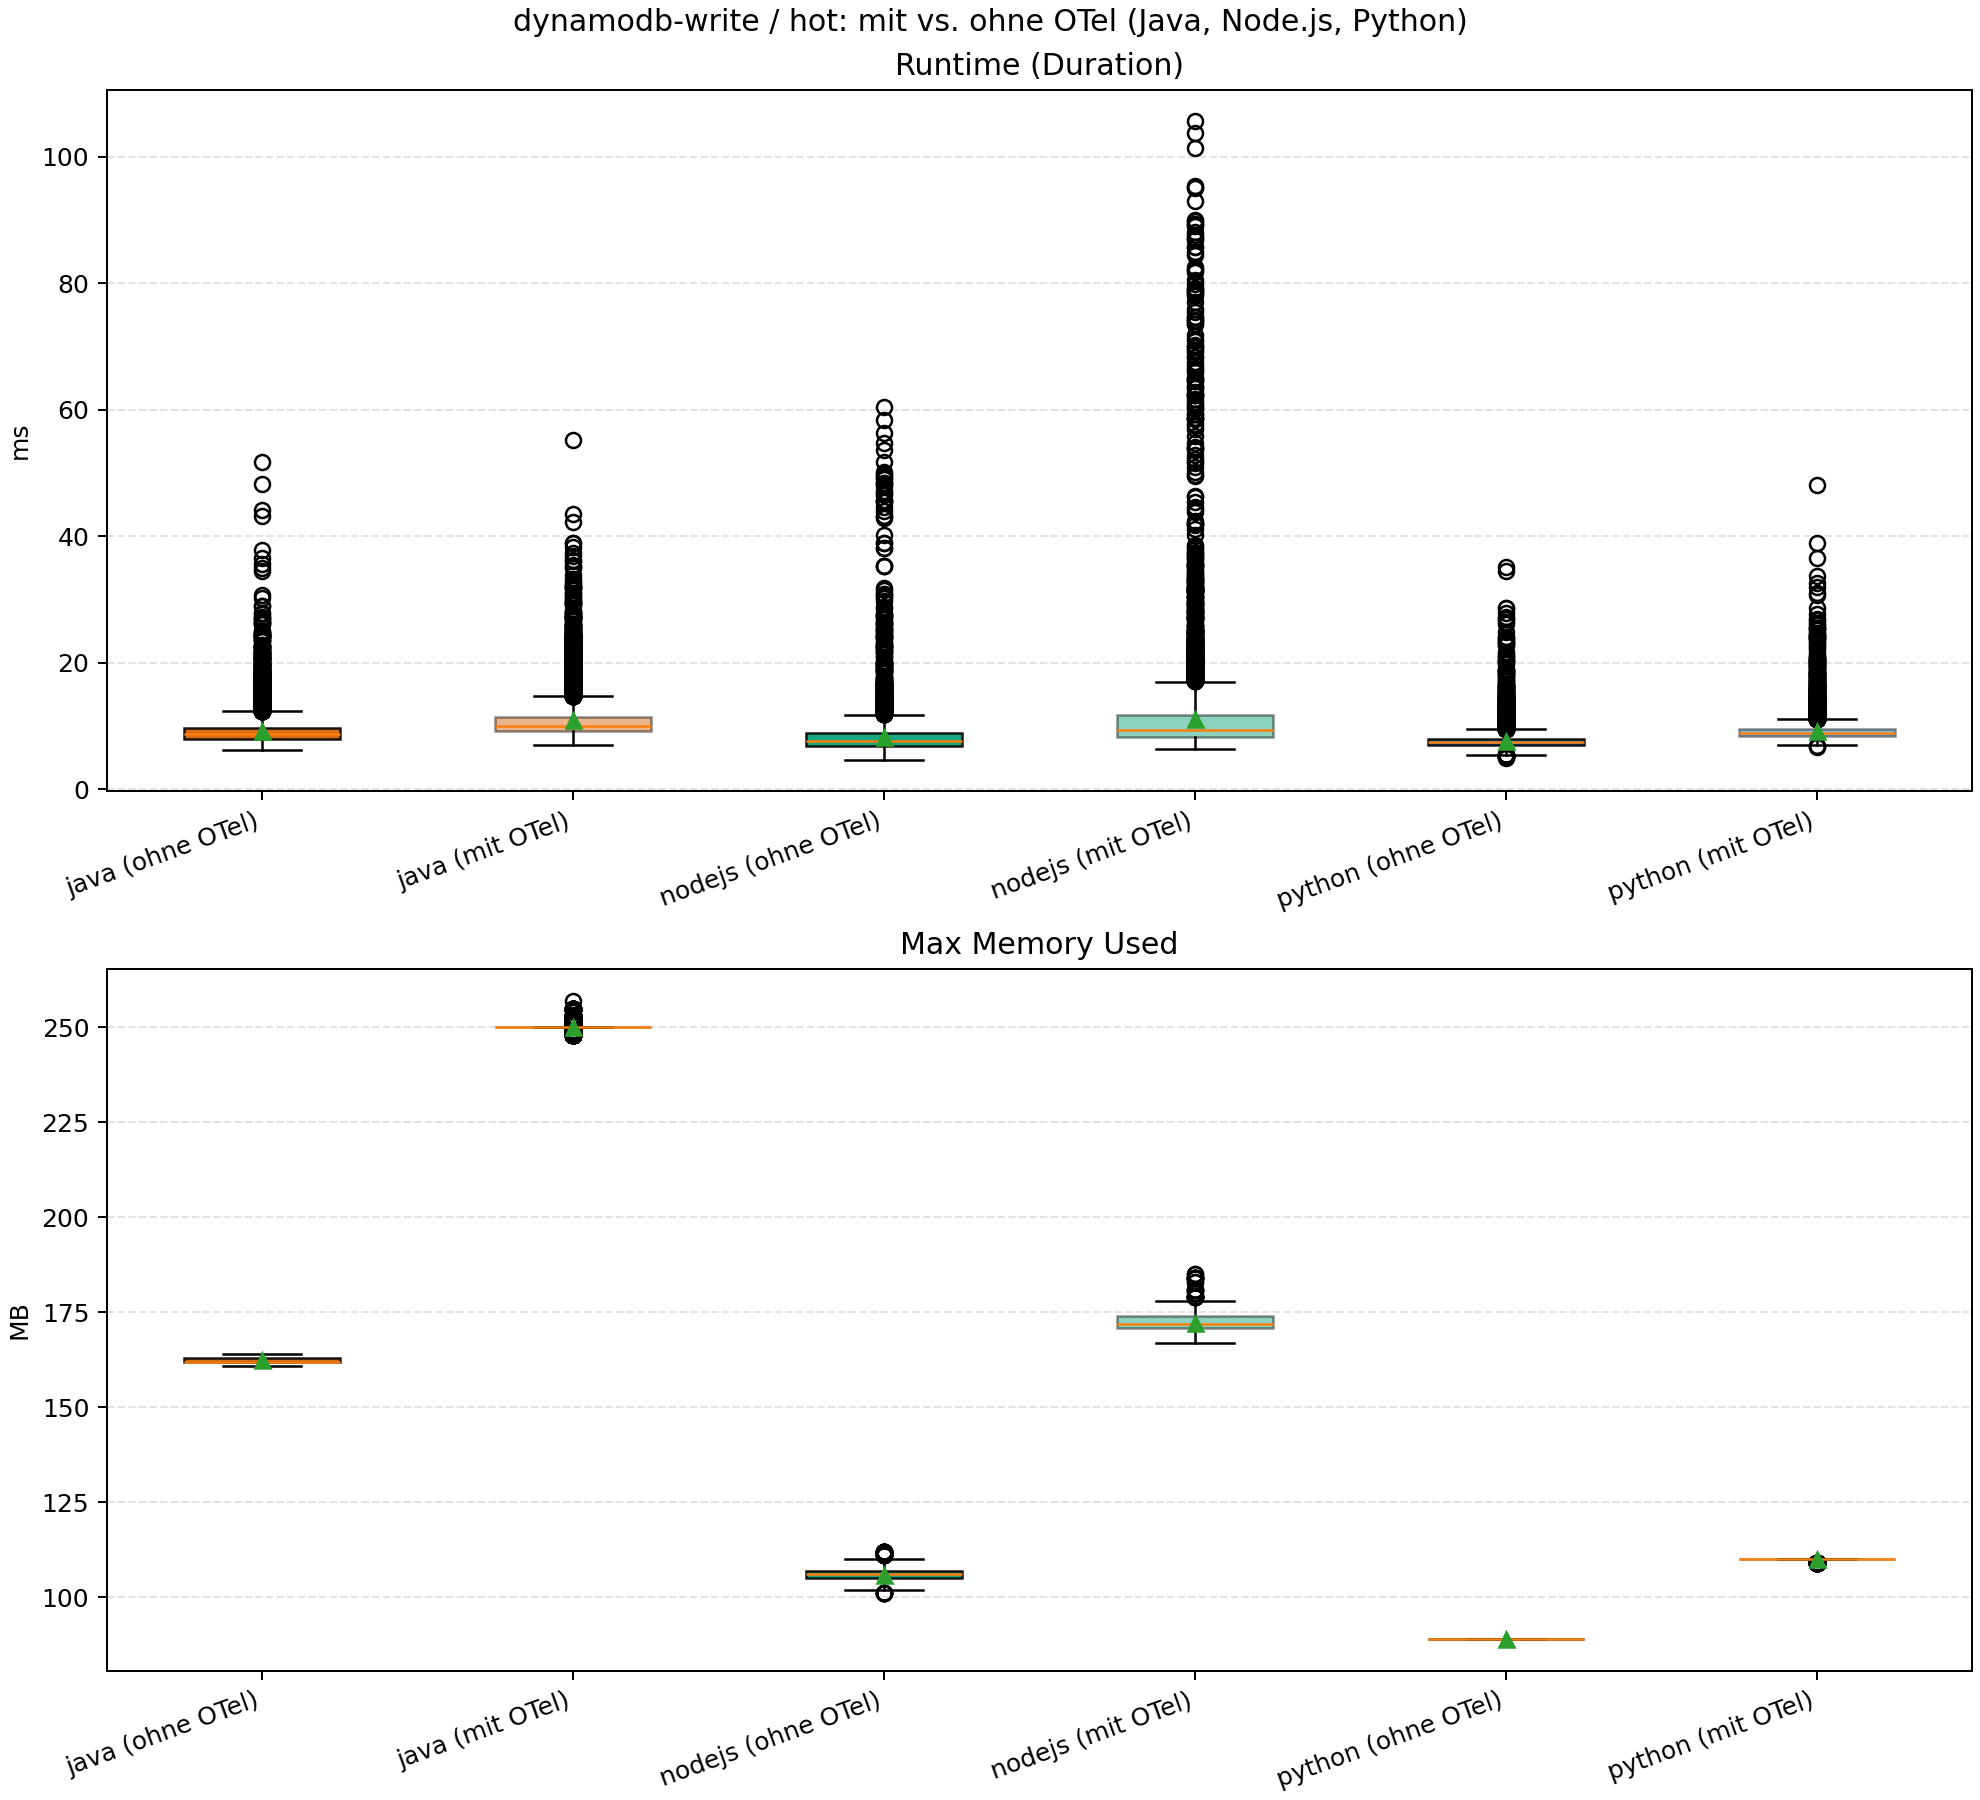
\includegraphics[width=1\textwidth]{./gfx/examples/dynamodb-write-hot-otel-comparison.png}
    \caption{Verteilung der Warmstartergebnisse für die DynamoDB-Schreibeoperation.}
    \label{fig:dynamodb-write-hot-otel-comparison}
\end{figure}

\section {Messergebnisse und Hypothesentests im Detail}
\label{sec:messwerte-im-detail}

\subsection{Rohe Messergebnisse}

\subsection{Ergebnisse der Bootstrap-Tests}

\section{Ranglisten der Sprachen}

\subsection*{1. Ranglisten basierend auf dem prozentualen Overhead (Median)}
\label{app:ranking-overhead}

\subsubsection*{Kaltstarts}

% Init Duration
\begin{table}[H]
\centering
\begin{minipage}{0.45\textwidth}
\centering
\caption{Bootstrap (Median) – Init Duration (5 Vergleiche)}
\begin{tabular}{|l|ccc|}
\hline
Sprache & 1. & 2. & 3. \\
\hline
Java    & 2 & 3 & 0 \\
Node.js & 0 & 0 & 5 \\
Python  & 3 & 2 & 0 \\
\hline
\end{tabular}
\end{minipage}\hfill
\begin{minipage}{0.45\textwidth}
\centering
\caption{Originaldaten (Median) – Init Duration (5 Vergleiche)}
\begin{tabular}{|l|ccc|}
\hline
Sprache & 1. & 2. & 3. \\
\hline
Java    & 0 & 3 & 2 \\
Node.js & 2 & 0 & 3 \\
Python  & 3 & 2 & 0 \\
\hline
\end{tabular}
\end{minipage}
\end{table}

% Duration
\begin{table}[H]
\centering
\begin{minipage}{0.45\textwidth}
\centering
\caption{Bootstrap – Duration (5 Vergleiche)}
\begin{tabular}{|l|ccc|}
\hline
Sprache & 1. & 2. & 3. \\
\hline
Java    & 0 & 3 & 2 \\
Node.js & 2 & 0 & 3 \\
Python  & 3 & 2 & 0 \\
\hline
\end{tabular}
\end{minipage}\hfill
\begin{minipage}{0.45\textwidth}
\centering
\caption{Originaldaten – Duration (5 Vergleiche)}
\begin{tabular}{|l|ccc|}
\hline
Sprache & 1. & 2. & 3. \\
\hline
Java    & 0 & 3 & 2 \\
Node.js & 2 & 0 & 3 \\
Python  & 3 & 2 & 0 \\
\hline
\end{tabular}
\end{minipage}
\end{table}

% Max Memory
\begin{table}[H]
\centering
\begin{minipage}{0.45\textwidth}
\centering
\caption{Bootstrap – Max Memory (5 Vergleiche)}
\begin{tabular}{|l|ccc|}
\hline
Sprache & 1. & 2. & 3. \\
\hline
Java    & 2 & 3 & 0 \\
Node.js & 0 & 0 & 5 \\
Python  & 3 & 2 & 0 \\
\hline
\end{tabular}
\end{minipage}\hfill
\begin{minipage}{0.45\textwidth}
\centering
\caption{Originaldaten – Max Memory (5 Vergleiche)}
\begin{tabular}{|l|ccc|}
\hline
Sprache & 1. & 2. & 3. \\
\hline
Java    & 0 & 0 & 5 \\
Node.js & 0 & 5 & 0 \\
Python  & 5 & 0 & 0 \\
\hline
\end{tabular}
\end{minipage}
\end{table}

% Kombiniert Kalt
\begin{table}[H]
\centering
\begin{minipage}{0.45\textwidth}
\centering
\caption{Bootstrap – Kombiniert Kalt (15 Vergleiche)}
\begin{tabular}{|l|ccc|}
\hline
Sprache & 1. & 2. & 3. \\
\hline
Java    & 4 & 9 & 2 \\
Node.js & 2 & 0 & 13 \\
Python  & 9 & 6 & 0 \\
\hline
\end{tabular}
\end{minipage}\hfill
\begin{minipage}{0.45\textwidth}
\centering
\caption{Originaldaten – Kombiniert Kalt (15 Vergleiche)}
\begin{tabular}{|l|ccc|}
\hline
Sprache & 1. & 2. & 3. \\
\hline
Java    & 0 & 6 & 9 \\
Node.js & 4 & 5 & 6 \\
Python  & 11 & 4 & 0 \\
\hline
\end{tabular}
\end{minipage}
\end{table}

\subsubsection*{Warmstarts}

% Duration Warm
\begin{table}[H]
\centering
\begin{minipage}{0.45\textwidth}
\centering
\caption{Bootstrap – Duration (5 Vergleiche)}
\begin{tabular}{|l|ccc|}
\hline
Sprache & 1. & 2. & 3. \\
\hline
Java    & 3 & 2 & 0 \\
Node.js & 2 & 0 & 3 \\
Python  & 0 & 3 & 2 \\
\hline
\end{tabular}
\end{minipage}\hfill
\begin{minipage}{0.45\textwidth}
\centering
\caption{Originaldaten – Duration (5 Vergleiche)}
\begin{tabular}{|l|ccc|}
\hline
Sprache & 1. & 2. & 3. \\
\hline
Java    & 3 & 2 & 0 \\
Node.js & 2 & 0 & 3 \\
Python  & 0 & 3 & 2 \\
\hline
\end{tabular}
\end{minipage}
\end{table}

% Max Memory Warm
\begin{table}[H]
\centering
\begin{minipage}{0.45\textwidth}
\centering
\caption{Bootstrap – Max Memory (5 Vergleiche)}
\begin{tabular}{|l|ccc|}
\hline
Sprache & 1. & 2. & 3. \\
\hline
Java    & 1 & 4 & 0 \\
Node.js & 1 & 1 & 3 \\
Python  & 3 & 0 & 2 \\
\hline
\end{tabular}
\end{minipage}\hfill
\begin{minipage}{0.45\textwidth}
\centering
\caption{Originaldaten – Max Memory (5 Vergleiche)}
\begin{tabular}{|l|ccc|}
\hline
Sprache & 1. & 2. & 3. \\
\hline
Java    & 0 & 0 & 5 \\
Node.js & 0 & 5 & 0 \\
Python  & 5 & 0 & 0 \\
\hline
\end{tabular}
\end{minipage}
\end{table}

% Kombiniert Warm
\begin{table}[H]
\centering
\begin{minipage}{0.45\textwidth}
\centering
\caption{Bootstrap – Kombiniert Warm (10 Vergleiche)}
\begin{tabular}{|l|ccc|}
\hline
Sprache & 1. & 2. & 3. \\
\hline
Java    & 4 & 6 & 0 \\
Node.js & 3 & 1 & 6 \\
Python  & 3 & 3 & 4 \\
\hline
\end{tabular}
\end{minipage}\hfill
\begin{minipage}{0.45\textwidth}
\centering
\caption{Originaldaten – Kombiniert Warm (10 Vergleiche)}
\begin{tabular}{|l|ccc|}
\hline
Sprache & 1. & 2. & 3. \\
\hline
Java    & 3 & 2 & 5 \\
Node.js & 2 & 5 & 3 \\
Python  & 5 & 3 & 2 \\
\hline
\end{tabular}
\end{minipage}
\end{table}

% Combined gesamt (25)
\begin{table}[H]
\centering
\begin{minipage}{0.45\textwidth}
\centering
\caption{Bootstrap – gesamt (25 Vergleiche)}
\begin{tabular}{|l|ccc|}
\hline
Sprache & 1. & 2. & 3. \\
\hline
Java    & 8 & 15 & 2 \\
Node.js & 5 & 1 & 19 \\
Python  & 12 & 9 & 4 \\
\hline
\end{tabular}
\end{minipage}\hfill
\begin{minipage}{0.45\textwidth}
\centering
\caption{Originaldaten – gesamt (25 Vergleiche)}
\begin{tabular}{|l|ccc|}
\hline
Sprache & 1. & 2. & 3. \\
\hline
Java    & 3 & 8 & 14 \\
Node.js & 6 & 10 & 9 \\
Python  & 16 & 7 & 2 \\
\hline
\end{tabular}
\end{minipage}
\end{table}

\newpage
\subsection*{2. Ranglisten basierend auf absoluten Messwerten ohne OpenTelemetry}
\label{app:ranking-without-otel}

\subsubsection*{Kaltstarts}

% Init Duration
\begin{table}[H]
\centering
\begin{minipage}{0.45\textwidth}
\centering
\caption{Bootstrap – Init Duration (5 Vergleiche)}
\begin{tabular}{|l|ccc|}
\hline
Sprache & 1. & 2. & 3. \\
\hline
Java    & 0 & 0 & 5 \\
Node.js & 5 & 0 & 0 \\
Python  & 0 & 5 & 0 \\
\hline
\end{tabular}
\end{minipage}\hfill
\begin{minipage}{0.45\textwidth}
\centering
\caption{Originaldaten – Init Duration (5 Vergleiche)}
\begin{tabular}{|l|ccc|}
\hline
Sprache & 1. & 2. & 3. \\
\hline
Java    & 0 & 0 & 5 \\
Node.js & 5 & 0 & 0 \\
Python  & 0 & 5 & 0 \\
\hline
\end{tabular}
\end{minipage}
\end{table}

% Duration
\begin{table}[H]
\centering
\begin{minipage}{0.45\textwidth}
\centering
\caption{Bootstrap – Duration (5 Vergleiche)}
\begin{tabular}{|l|ccc|}
\hline
Sprache & 1. & 2. & 3. \\
\hline
Java    & 0 & 0 & 5 \\
Node.js & 0 & 5 & 0 \\
Python  & 5 & 0 & 0 \\
\hline
\end{tabular}
\end{minipage}\hfill
\begin{minipage}{0.45\textwidth}
\centering
\caption{Originaldaten – Duration (5 Vergleiche)}
\begin{tabular}{|l|ccc|}
\hline
Sprache & 1. & 2. & 3. \\
\hline
Java    & 0 & 0 & 5 \\
Node.js & 0 & 5 & 0 \\
Python  & 5 & 0 & 0 \\
\hline
\end{tabular}
\end{minipage}
\end{table}

% Max Memory
\begin{table}[H]
\centering
\begin{minipage}{0.45\textwidth}
\centering
\caption{Bootstrap – Max Memory (5 Vergleiche)}
\begin{tabular}{|l|ccc|}
\hline
Sprache & 1. & 2. & 3. \\
\hline
Java    & 0 & 0 & 5 \\
Node.js & 0 & 5 & 0 \\
Python  & 5 & 0 & 0 \\
\hline
\end{tabular}
\end{minipage}\hfill
\begin{minipage}{0.45\textwidth}
\centering
\caption{Originaldaten – Max Memory (5 Vergleiche)}
\begin{tabular}{|l|ccc|}
\hline
Sprache & 1. & 2. & 3. \\
\hline
Java    & 0 & 0 & 5 \\
Node.js & 0 & 5 & 0 \\
Python  & 5 & 0 & 0 \\
\hline
\end{tabular}
\end{minipage}
\end{table}

% Kombiniert Kalt
\begin{table}[H]
\centering
\begin{minipage}{0.45\textwidth}
\centering
\caption{Bootstrap – Kombiniert Kalt (15 Vergleiche)}
\begin{tabular}{|l|ccc|}
\hline
Sprache & 1. & 2. & 3. \\
\hline
Java    & 0 & 0 & 15 \\
Node.js & 5 & 10 & 0 \\
Python  & 10 & 5 & 0 \\
\hline
\end{tabular}
\end{minipage}\hfill
\begin{minipage}{0.45\textwidth}
\centering
\caption{Originaldaten – Kombiniert Kalt (15 Vergleiche)}
\begin{tabular}{|l|ccc|}
\hline
Sprache & 1. & 2. & 3. \\
\hline
Java    & 0 & 0 & 15 \\
Node.js & 5 & 10 & 0 \\
Python  & 10 & 5 & 0 \\
\hline
\end{tabular}
\end{minipage}
\end{table}

\subsubsection*{Warmstarts}

% Duration
\begin{table}[H]
\centering
\begin{minipage}{0.45\textwidth}
\centering
\caption{Bootstrap – Duration (5 Vergleiche)}
\begin{tabular}{|l|ccc|}
\hline
Sprache & 1. & 2. & 3. \\
\hline
Java    & 0 & 3 & 2 \\
Node.js & 1 & 2 & 2 \\
Python  & 4 & 0 & 1 \\
\hline
\end{tabular}
\end{minipage}\hfill
\begin{minipage}{0.45\textwidth}
\centering
\caption{Originaldaten – Duration (5 Vergleiche)}
\begin{tabular}{|l|ccc|}
\hline
Sprache & 1. & 2. & 3. \\
\hline
Java    & 0 & 3 & 2 \\
Node.js & 1 & 2 & 2 \\
Python  & 4 & 0 & 1 \\
\hline
\end{tabular}
\end{minipage}
\end{table}

% Max Memory
\begin{table}[H]
\centering
\begin{minipage}{0.45\textwidth}
\centering
\caption{Bootstrap – Max Memory (5 Vergleiche)}
\begin{tabular}{|l|ccc|}
\hline
Sprache & 1. & 2. & 3. \\
\hline
Java    & 0 & 0 & 5 \\
Node.js & 0 & 5 & 0 \\
Python  & 5 & 0 & 0 \\
\hline
\end{tabular}
\end{minipage}\hfill
\begin{minipage}{0.45\textwidth}
\centering
\caption{Originaldaten – Max Memory (5 Vergleiche)}
\begin{tabular}{|l|ccc|}
\hline
Sprache & 1. & 2. & 3. \\
\hline
Java    & 0 & 0 & 5 \\
Node.js & 0 & 5 & 0 \\
Python  & 5 & 0 & 0 \\
\hline
\end{tabular}
\end{minipage}
\end{table}

% Kombiniert Warm
\begin{table}[H]
\centering
\begin{minipage}{0.45\textwidth}
\centering
\caption{Bootstrap – Kombiniert Warm (10 Vergleiche)}
\begin{tabular}{|l|ccc|}
\hline
Sprache & 1. & 2. & 3. \\
\hline
Java    & 0 & 3 & 7 \\
Node.js & 1 & 7 & 2 \\
Python  & 9 & 0 & 1 \\
\hline
\end{tabular}
\end{minipage}\hfill
\begin{minipage}{0.45\textwidth}
\centering
\caption{Originaldaten – Kombiniert Warm (10 Vergleiche)}
\begin{tabular}{|l|ccc|}
\hline
Sprache & 1. & 2. & 3. \\
\hline
Java    & 0 & 3 & 7 \\
Node.js & 1 & 7 & 2 \\
Python  & 9 & 0 & 1 \\
\hline
\end{tabular}
\end{minipage}
\end{table}

% Combined gesamt
\begin{table}[H]
\centering
\begin{minipage}{0.45\textwidth}
\centering
\caption{Bootstrap – gesamt (25 Vergleiche)}
\begin{tabular}{|l|ccc|}
\hline
Sprache & 1. & 2. & 3. \\
\hline
Java    & 0 & 3 & 22 \\
Node.js & 6 & 17 & 2 \\
Python  & 19 & 5 & 1 \\
\hline
\end{tabular}
\end{minipage}\hfill
\begin{minipage}{0.45\textwidth}
\centering
\caption{Originaldaten – gesamt (25 Vergleiche)}
\begin{tabular}{|l|ccc|}
\hline
Sprache & 1. & 2. & 3. \\
\hline
Java    & 0 & 3 & 22 \\
Node.js & 6 & 17 & 2 \\
Python  & 19 & 5 & 1 \\
\hline
\end{tabular}
\end{minipage}
\end{table}

\subsection*{3. Ranglisten basierend auf absoluten Messwerten mit OpenTelemetry}
\label{app:ranking-with-otel}

\subsubsection*{Kaltstarts}

% Init Duration
\begin{table}[H]
\centering
\begin{minipage}{0.45\textwidth}
\centering
\caption{Bootstrap – Init Duration (5 Vergleiche)}
\begin{tabular}{|l|ccc|}
\hline
Sprache & 1. & 2. & 3. \\
\hline
Java    & 0 & 0 & 5 \\
Node.js & 0 & 5 & 0 \\
Python  & 5 & 0 & 0 \\
\hline
\end{tabular}
\end{minipage}\hfill
\begin{minipage}{0.45\textwidth}
\centering
\caption{Originaldaten – Init Duration (5 Vergleiche)}
\begin{tabular}{|l|ccc|}
\hline
Sprache & 1. & 2. & 3. \\
\hline
Java    & 0 & 0 & 5 \\
Node.js & 0 & 5 & 0 \\
Python  & 5 & 0 & 0 \\
\hline
\end{tabular}
\end{minipage}
\end{table}

% Duration
\begin{table}[H]
\centering
\begin{minipage}{0.45\textwidth}
\centering
\caption{Bootstrap – Duration (5 Vergleiche)}
\begin{tabular}{|l|ccc|}
\hline
Sprache & 1. & 2. & 3. \\
\hline
Java    & 0 & 0 & 5 \\
Node.js & 0 & 5 & 0 \\
Python  & 5 & 0 & 0 \\
\hline
\end{tabular}
\end{minipage}\hfill
\begin{minipage}{0.45\textwidth}
\centering
\caption{Originaldaten – Duration (5 Vergleiche)}
\begin{tabular}{|l|ccc|}
\hline
Sprache & 1. & 2. & 3. \\
\hline
Java    & 0 & 0 & 5 \\
Node.js & 0 & 5 & 0 \\
Python  & 5 & 0 & 0 \\
\hline
\end{tabular}
\end{minipage}
\end{table}

% Max Memory
\begin{table}[H]
\centering
\begin{minipage}{0.45\textwidth}
\centering
\caption{Bootstrap – Max Memory (5 Vergleiche)}
\begin{tabular}{|l|ccc|}
\hline
Sprache & 1. & 2. & 3. \\
\hline
Java    & 0 & 0 & 5 \\
Node.js & 0 & 5 & 0 \\
Python  & 5 & 0 & 0 \\
\hline
\end{tabular}
\end{minipage}\hfill
\begin{minipage}{0.45\textwidth}
\centering
\caption{Originaldaten – Max Memory (5 Vergleiche)}
\begin{tabular}{|l|ccc|}
\hline
Sprache & 1. & 2. & 3. \\
\hline
Java    & 0 & 0 & 5 \\
Node.js & 0 & 5 & 0 \\
Python  & 5 & 0 & 0 \\
\hline
\end{tabular}
\end{minipage}
\end{table}

% Kombiniert Kalt
\begin{table}[H]
\centering
\begin{minipage}{0.45\textwidth}
\centering
\caption{Bootstrap – Kombiniert Kalt (15 Vergleiche)}
\begin{tabular}{|l|ccc|}
\hline
Sprache & 1. & 2. & 3. \\
\hline
Java    & 0 & 0 & 15 \\
Node.js & 0 & 15 & 0 \\
Python  & 15 & 0 & 0 \\
\hline
\end{tabular}
\end{minipage}\hfill
\begin{minipage}{0.45\textwidth}
\centering
\caption{Originaldaten – Kombiniert Kalt (15 Vergleiche)}
\begin{tabular}{|l|ccc|}
\hline
Sprache & 1. & 2. & 3. \\
\hline
Java    & 0 & 0 & 15 \\
Node.js & 0 & 15 & 0 \\
Python  & 15 & 0 & 0 \\
\hline
\end{tabular}
\end{minipage}
\end{table}

\subsubsection*{Warmstarts}

% Duration
\begin{table}[H]
\centering
\begin{minipage}{0.45\textwidth}
\centering
\caption{Bootstrap – Duration (5 Vergleiche)}
\begin{tabular}{|l|ccc|}
\hline
Sprache & 1. & 2. & 3. \\
\hline
Java    & 1 & 1 & 3 \\
Node.js & 0 & 4 & 1 \\
Python  & 4 & 0 & 1 \\
\hline
\end{tabular}
\end{minipage}\hfill
\begin{minipage}{0.45\textwidth}
\centering
\caption{Originaldaten – Duration (5 Vergleiche)}
\begin{tabular}{|l|ccc|}
\hline
Sprache & 1. & 2. & 3. \\
\hline
Java    & 1 & 1 & 3 \\
Node.js & 0 & 4 & 1 \\
Python  & 4 & 0 & 1 \\
\hline
\end{tabular}
\end{minipage}
\end{table}

% Max Memory
\begin{table}[H]
\centering
\begin{minipage}{0.45\textwidth}
\centering
\caption{Bootstrap – Max Memory (5 Vergleiche)}
\begin{tabular}{|l|ccc|}
\hline
Sprache & 1. & 2. & 3. \\
\hline
Java    & 0 & 0 & 5 \\
Node.js & 0 & 5 & 0 \\
Python  & 5 & 0 & 0 \\
\hline
\end{tabular}
\end{minipage}\hfill
\begin{minipage}{0.45\textwidth}
\centering
\caption{Originaldaten – Max Memory (5 Vergleiche)}
\begin{tabular}{|l|ccc|}
\hline
Sprache & 1. & 2. & 3. \\
\hline
Java    & 0 & 0 & 5 \\
Node.js & 0 & 5 & 0 \\
Python  & 5 & 0 & 0 \\
\hline
\end{tabular}
\end{minipage}
\end{table}

% Kombiniert Warm
\begin{table}[H]
\centering
\begin{minipage}{0.45\textwidth}
\centering
\caption{Bootstrap – Kombiniert Warm (10 Vergleiche)}
\begin{tabular}{|l|ccc|}
\hline
Sprache & 1. & 2. & 3. \\
\hline
Java    & 1 & 1 & 8 \\
Node.js & 0 & 9 & 1 \\
Python  & 9 & 0 & 1 \\
\hline
\end{tabular}
\end{minipage}\hfill
\begin{minipage}{0.45\textwidth}
\centering
\caption{Originaldaten – Kombiniert Warm (10 Vergleiche)}
\begin{tabular}{|l|ccc|}
\hline
Sprache & 1. & 2. & 3. \\
\hline
Java    & 1 & 1 & 8 \\
Node.js & 0 & 9 & 1 \\
Python  & 9 & 0 & 1 \\
\hline
\end{tabular}
\end{minipage}
\end{table}

% Combined gesamt
\begin{table}[H]
\centering
\begin{minipage}{0.45\textwidth}
\centering
\caption{Bootstrap – gesamt (25 Vergleiche)}
\begin{tabular}{|l|ccc|}
\hline
Sprache & 1. & 2. & 3. \\
\hline
Java    & 1 & 1 & 23 \\
Node.js & 0 & 24 & 1 \\
Python  & 24 & 0 & 1 \\
\hline
\end{tabular}
\end{minipage}\hfill
\begin{minipage}{0.45\textwidth}
\centering
\caption{Originaldaten – gesamt (25 Vergleiche)}
\begin{tabular}{|l|ccc|}
\hline
Sprache & 1. & 2. & 3. \\
\hline
Java    & 1 & 1 & 23 \\
Node.js & 0 & 24 & 1 \\
Python  & 24 & 0 & 1 \\
\hline
\end{tabular}
\end{minipage}
\end{table}